Neben der Bewertung des Spielfeldes \"ubernimmt der MapAnalyzer auch weitere Aufgaben.
Eine der Wichtigsten davon ist es herauszufinden, welche Felder erreichbar sind und welche nicht.

\subsection{Ablauf eines Analyse Vorgangs}\label{subsec:analyse-vorgang}
\subsubsection{Erreichbarkeit in ReversiXT}\label{subsubsec:erreichbarkeit}
In ReversiXT ist eine Reihe immer dann einnehmbar, wenn sich zwei Steine direkt nacheinander befinden.
Diese Erreichbarkeit breitet sich auch \"uber Transitionen hinweg aus und geht so lange, bis sie auf ein Loch oder sich selbst in gleicher Richtung st\"o"st.
Als Richtung versteht man dabei die Richtung, in die ein Feld verlassen wird, um in das n\"achste Feld zu gelangen.
Kleine Ver\"anderungen spielen bei der Erreichbarkeit eine gro"se Rolle.
So reicht es aus, einen Expansionsstein zu platzieren, um die gesamten erreichbaren Felder auf einer Karte zu ver\"andern.
Dies kann man im Abschnitt~\ref{paragraph:folgen-von-zuegen} nachvollziehen, bei dem durch einen Expansionsstein deutlich mehr Felder erreichbar werden.

\subsubsection{Logisches Vorgehen}\label{subsubsec:logisches-vorgehen}
Im Kapitel~\ref{subsubsec:erreichbarkeit} wird beschrieben, dass ein einzelner Stein sehr gro"se Auswirkungen darauf hat, ob es m\"oglich ist, eine ganze Karte zu bespielen oder nicht.
Um aber mit Sicherheit sagen zu k\"onnen, welche Bereiche erreichbar und welche unerreichbar sind, muss von jedem Feld aus nach neuen m\"oglichen Z\"ugen gesucht werden.
Im Folgenden wird der Vorgang der Kartenanalyse gezeigt.

\paragraph{Suchen der Startpunkte}
Dieser Schritt wirkt trivial, ist aber unabdingbar f\"ur eine erfolgreiche Analyse.
Indem man f\"ur jeden Spieler und Expansionsfeld in direkter N\"ahe nach m\"oglichen anderen Steinen zum \"uberziehen sucht, stellt man f\"ur alle Spieler die m\"oglichen Richtungen an Z\"ugen fest.
Dadurch k\"onnen zum Beispiel wie in der Abbildung~\ref{fig:unreachable} sogenannte \texttt{Inseln} ignoriert werden.
Diese k\"onnen w\"ahrend eines Spieles nie betreten werden, da sie weder Transitionen noch Expansionssteine besitzen.

\vspace{1em}
\begin{minipage}{\linewidth}
    \centering
    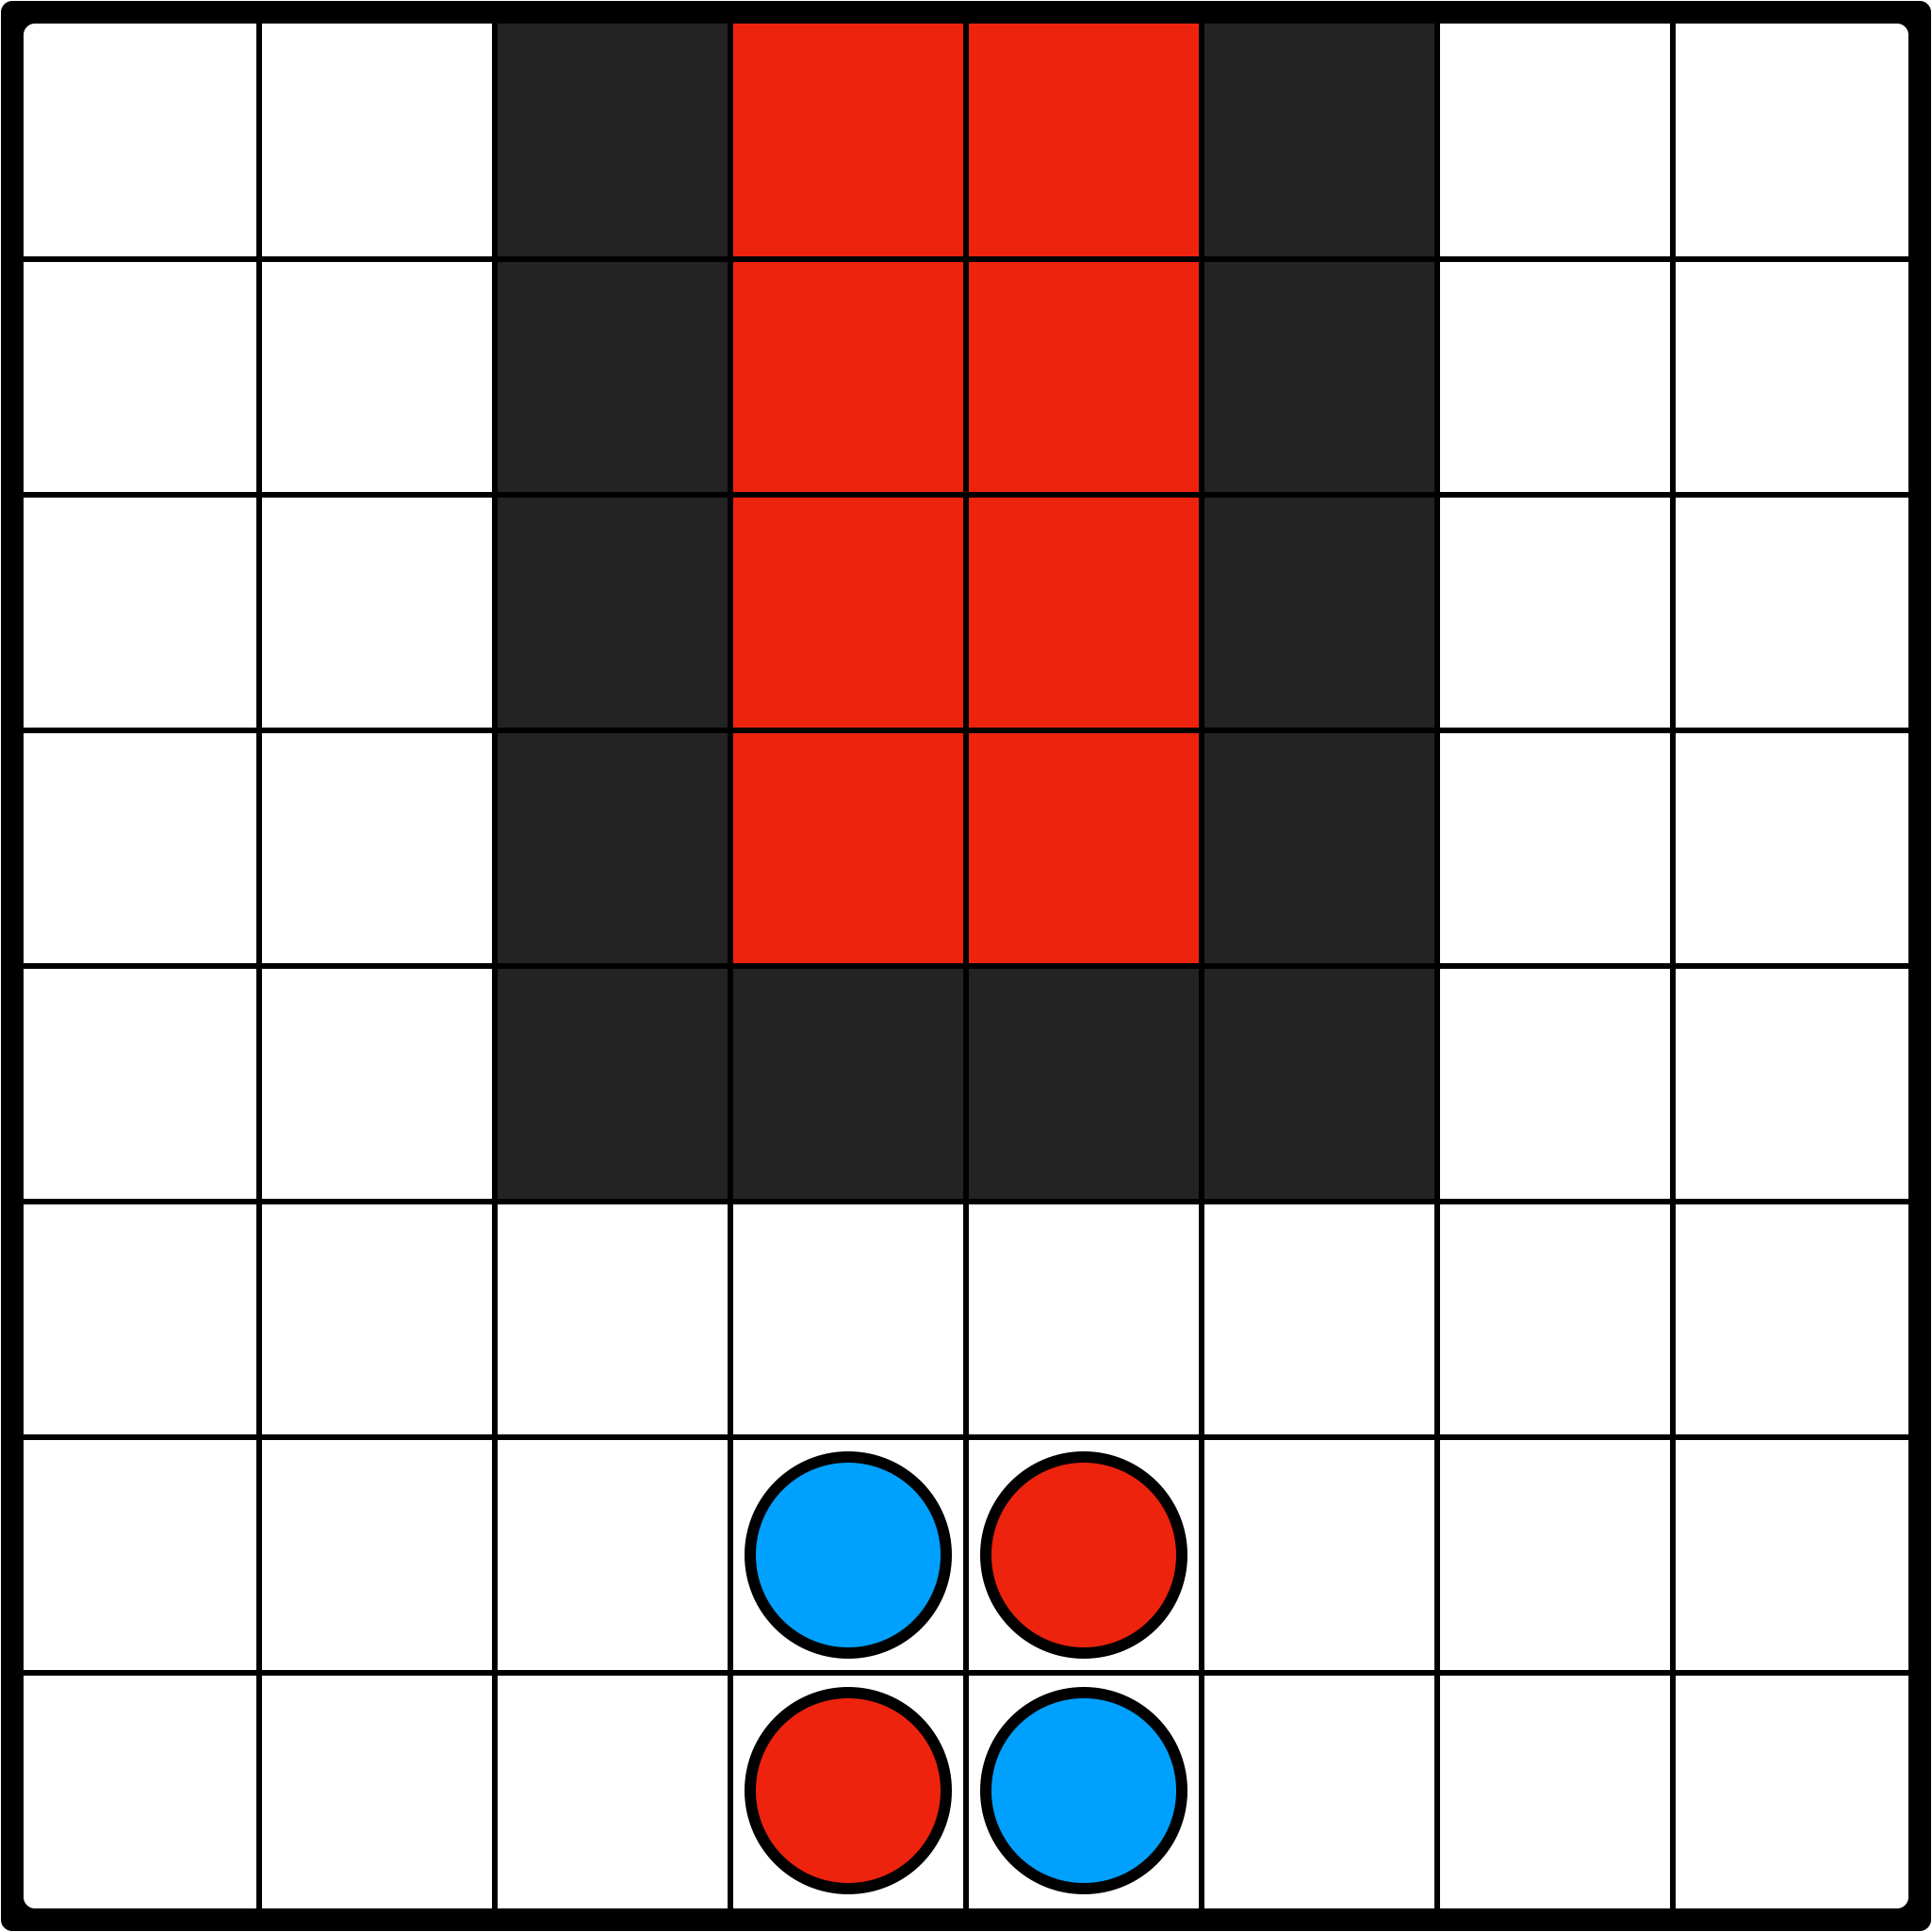
\includegraphics[width=0.45\linewidth]{pics/not-reachable}
    \captionof{figure}[Unerreichbarer Bereich]{Der rote Bereich ist vom MapAnalyzer als nicht erreichbar markiert.}
    \label{fig:unreachable}
\end{minipage}
\vspace{0.5em}

\paragraph{Folgen der m\"oglichen Z\"uge}\label{paragraph:folgen-von-zuegen}
\vspace{1em}
\begin{minipage}{\linewidth}
    \centering
    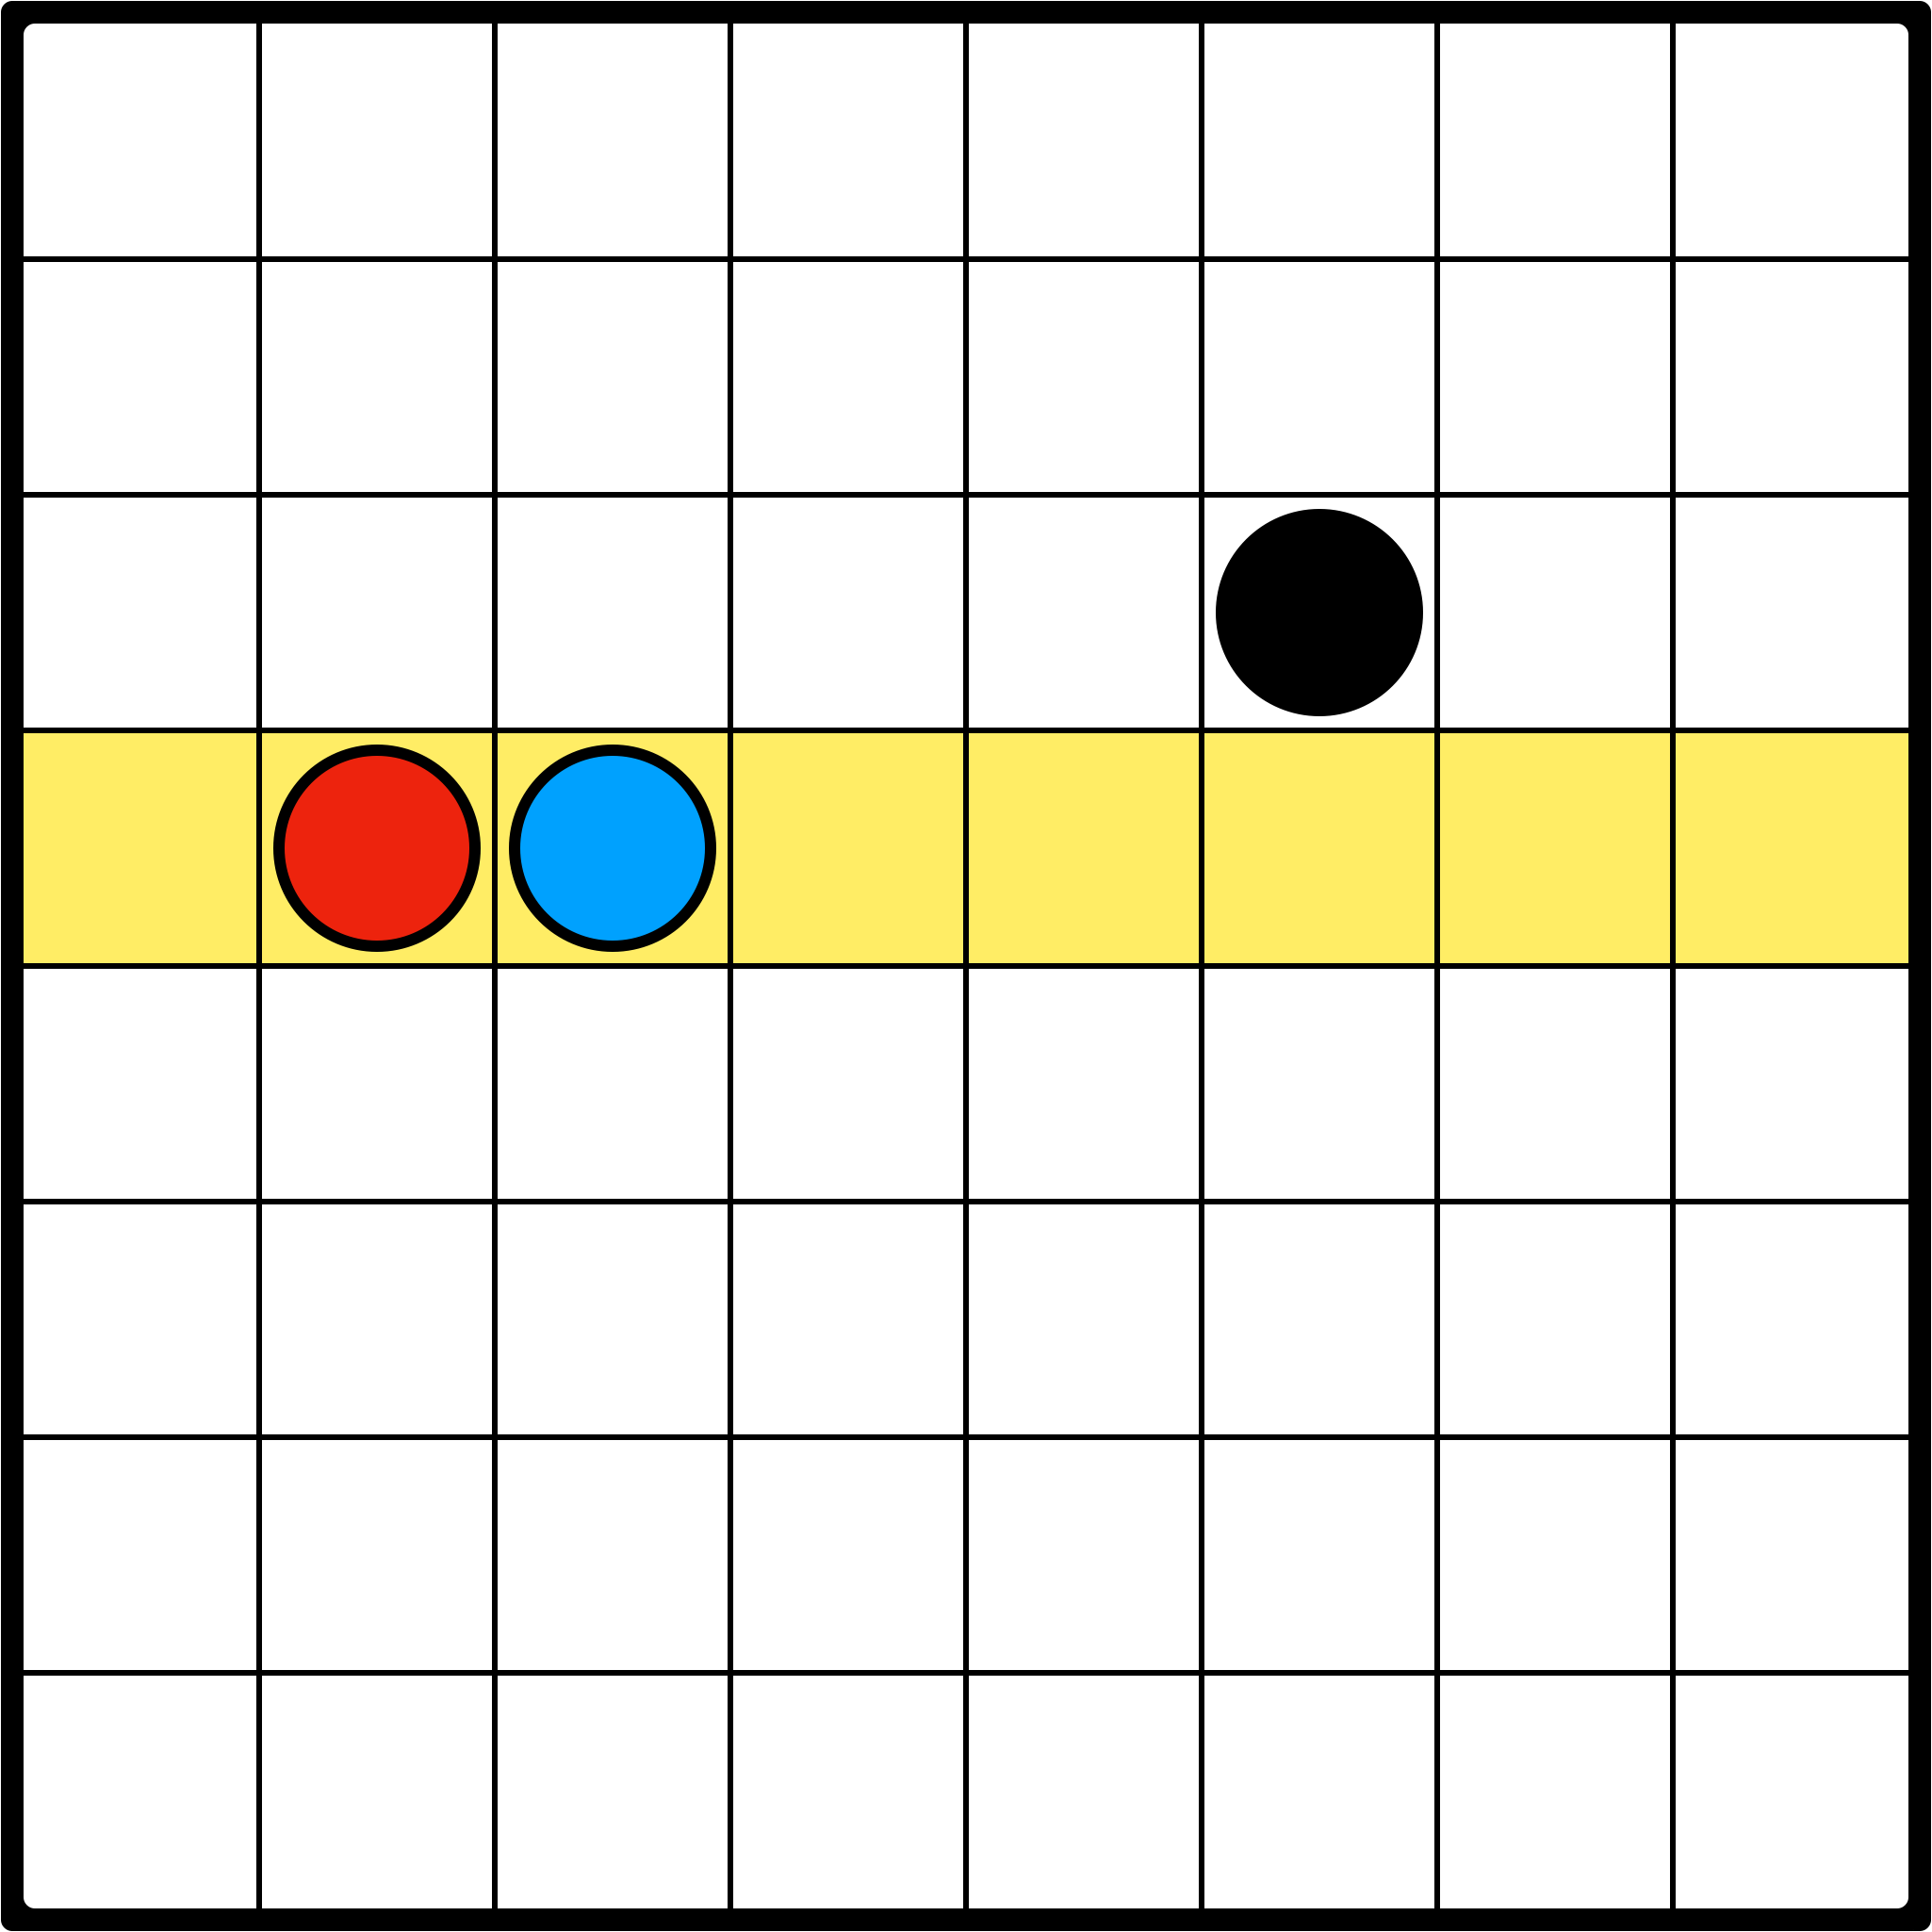
\includegraphics[width=0.45\linewidth]{pics/explaination/explaination-01}
    \captionof{figure}[Erkl\"arung 01]{Erste markierte Feldlinie in die der MapAnalyzer schaut.}
    \label{fig:explaination-01}
\end{minipage}
\vspace{0.5em}

Zu Beginn wird ein Stein gew\"ahlt, und in allen acht Richtungen nach m\"oglichen Z\"ugen gesucht.
Es wird also jedes direkt angrenzende Felde durchlaufen.
Falls sich nun in direkter N\"ahe ein anderer Spielerstein oder ein Expansionsstein befindet, ist in dieser, sowie in der entgegengesetzten Richtung ein Zug m\"oglich.
Somit kann die komplette Reihe erreicht werden.
Wieso Felder markiert werden m\"ussen wird im Kapitel~\ref{subsubsec:performance-probleme} genauer erkl\"art.
Markierte Felder sind hierbei Felder, die in einer sp\"ateren Iteration sicher noch erreicht werden.
Das folgende Bild zeigt die soeben erkl\"arten Vorg\"ange.

\vspace{1em}
\begin{minipage}{\linewidth}
    \centering
    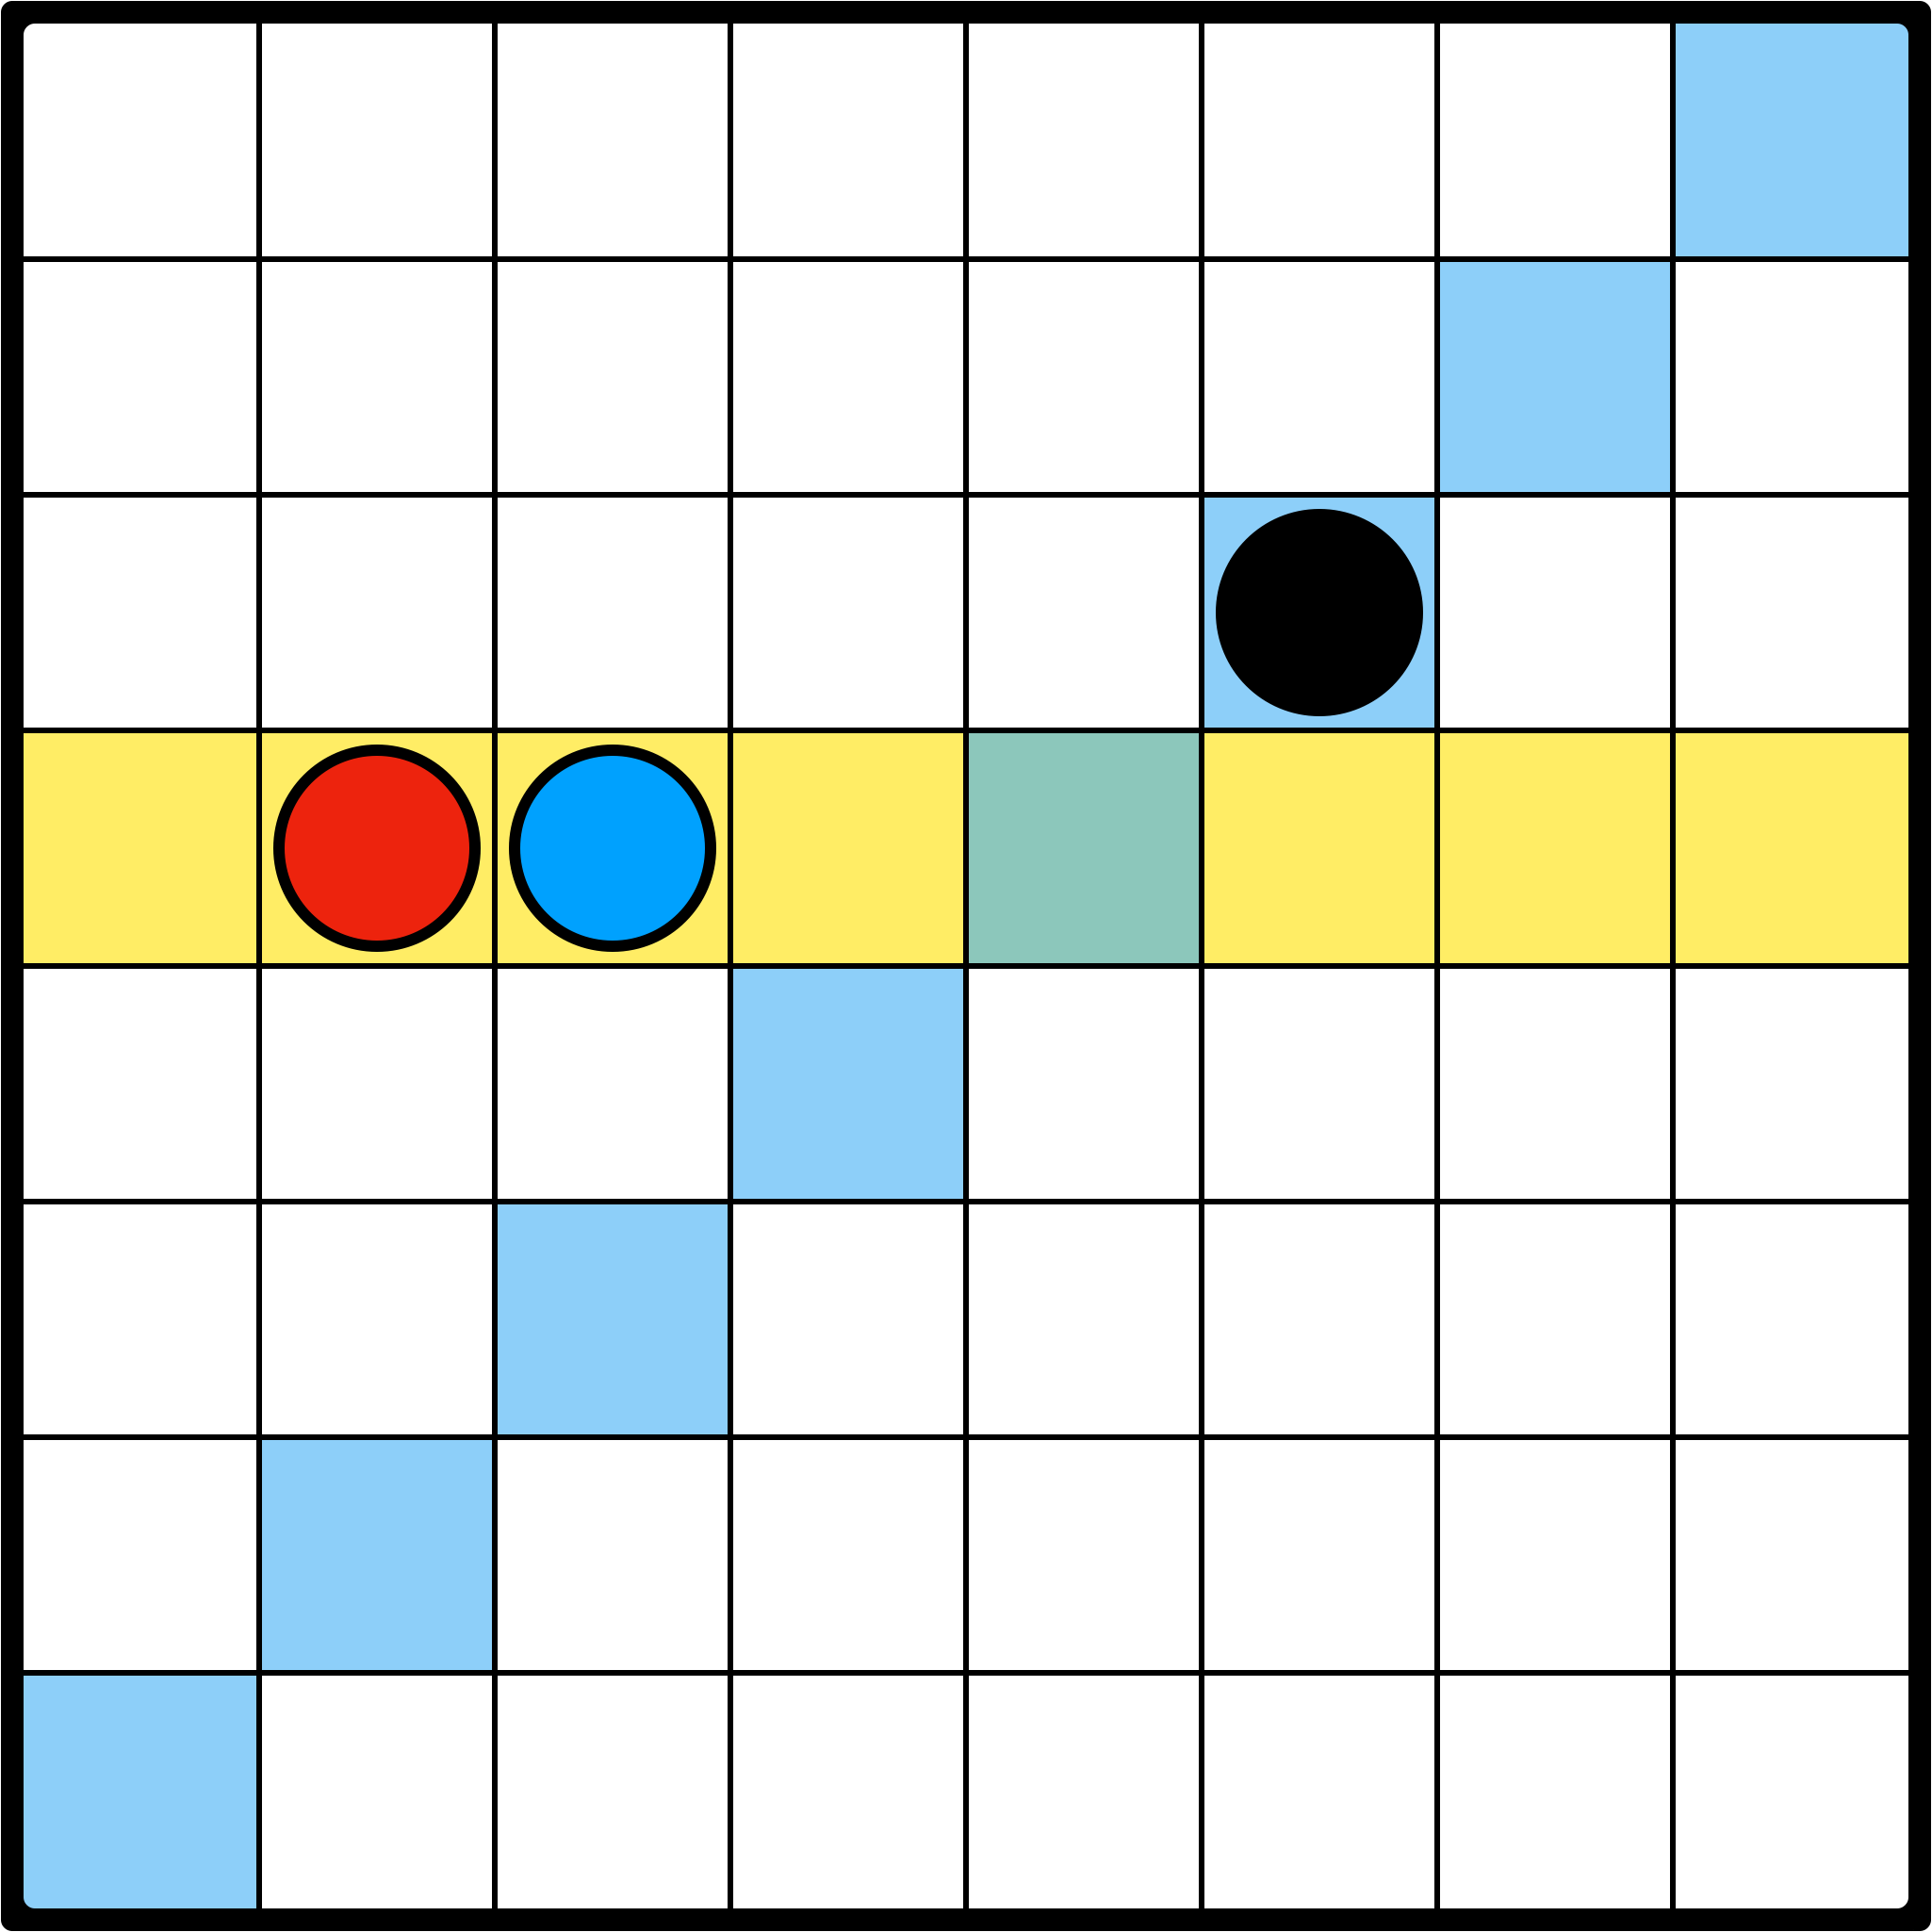
\includegraphics[width=0.45\linewidth]{pics/explaination/explaination-02}
    \captionof{figure}[Erkl\"arung 02]{Zweite markierte Feldlinie in die der MapAnalyzer schaut.}
    \label{fig:explaination-02}
\end{minipage}
\vspace{0.5em}

Sobald alle Felder markiert sind, wird weiter in die \"ubrigen Richtungen geschaut.
In diesem Beispiel existiert aber kein neuer Spielstein und damit gibt es keine neuen Z\"uge.
Die gleiche Logik gilt nun auch f\"ur die n\"achsten Steine in der aktuellen Reihe.

Bei den darauffolgenden Feldern werden nun wieder alle anliegenden Felder auf m\"ogliche Steine und damit m\"ogliche Z\"uge gepr\"uft.
Hier ist zu beachten, dass nicht auf Steine in der aktuellen Reihe geachtet wird, da diese sp\"ater noch abgearbeitet werden.
Zudem verhindert man damit unerw\"unschte Endlosschleifen.
Da in der darauffolgenden Iteration das Selbe wie eben passiert, wird diese \"ubersprungen.

In Abbildung~\ref{fig:explaination-02} wird bei der Analyse der benachbarten Felder ein Expansionsstein gefunden.
Demzufolge sind alle Felder in beide Richtungen erreichbar und werden markiert.

Nun wird dem neuen Pfad gefolgt und erneut in alle Richtungen nach Spielern gesucht.
Der m\"ogliche Weg \textit{nach unten} wird noch nicht erkannt, da markierte Felder nicht als m\"oglicher Zug z\"ahlen.
Anschlie"send wird dem blauen Pfad gefolgt.
In dieser Richtung st\"o"st man jedoch auf keine anliegenden Spieler, wodurch auch diese Iteration \"ubersprungen wird.

\vspace{1em}
\begin{minipage}{\linewidth}
    \centering
    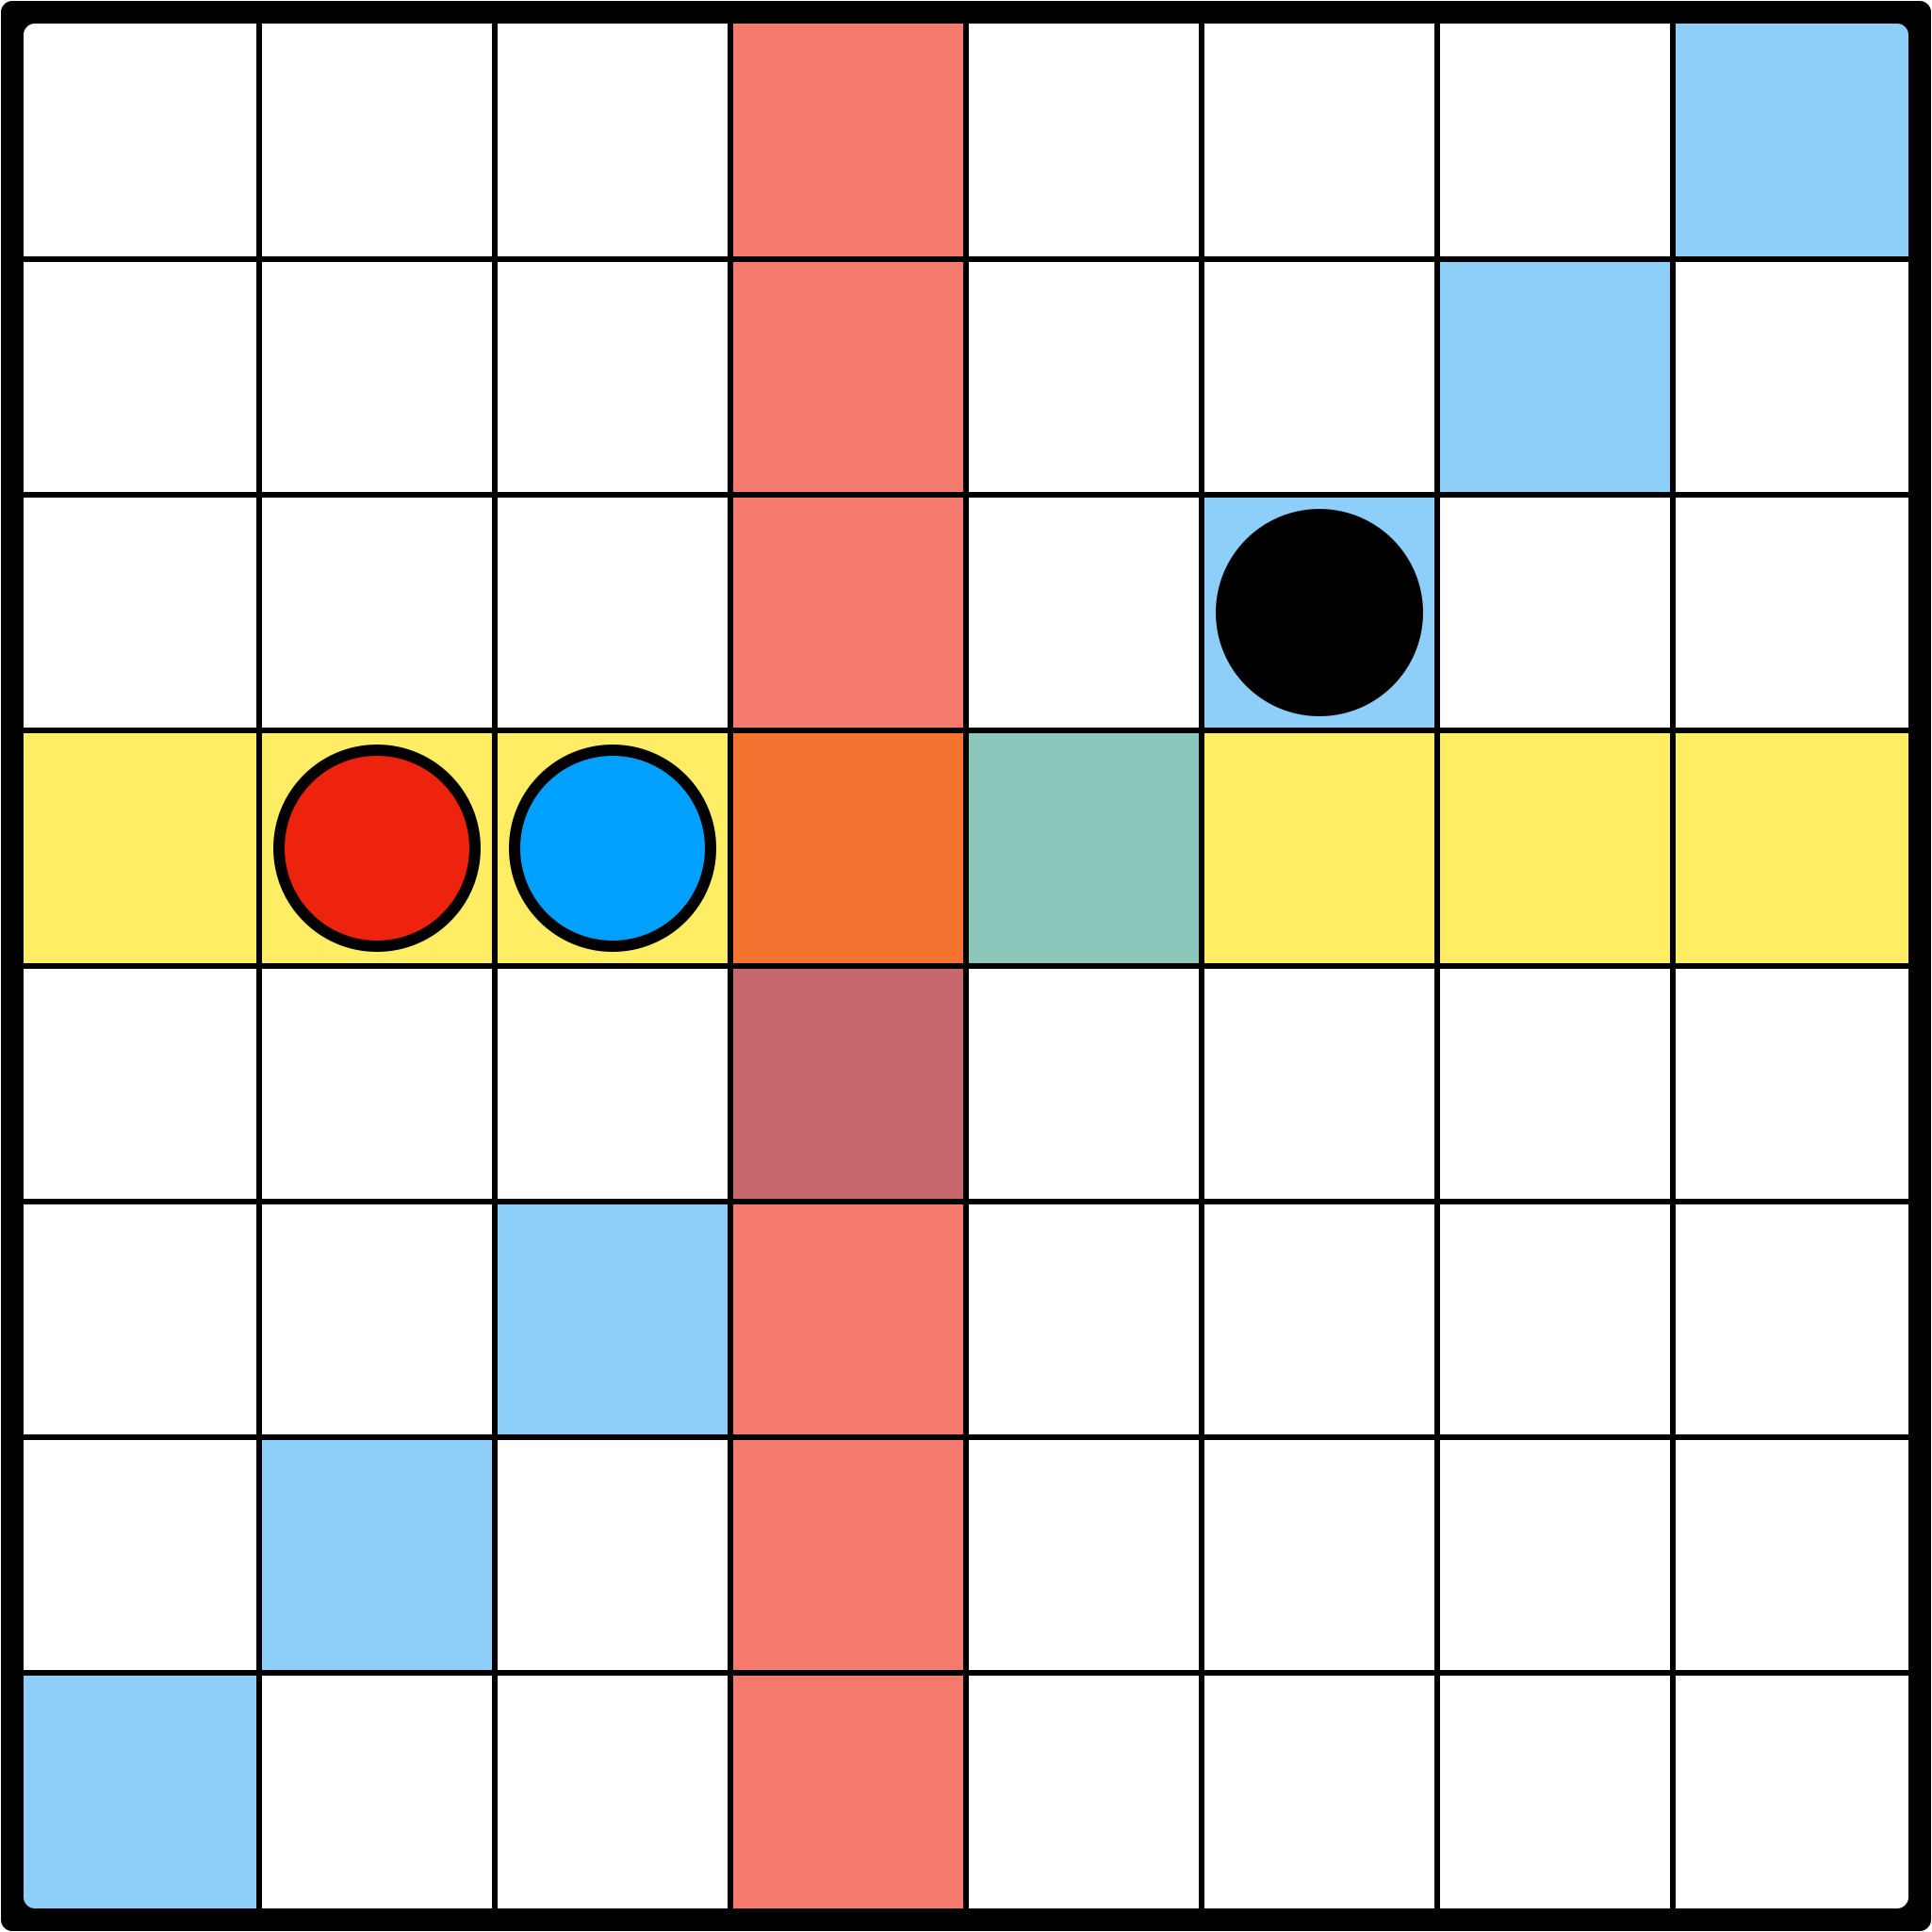
\includegraphics[width=0.45\linewidth]{pics/explaination/explaination-03}
    \captionof{figure}[Erkl\"arung 03]{Dritte markierte Feldlinie in die der MapAnalyzer schaut.}
    \label{fig:explaination-03}
\end{minipage}
\vspace{0.5em}

Wenn das eine Ende des blauen Pfades erreicht ist, wird nun die andere H\"alfte gepr\"uft.
Hierbei entsteht ein neuer Pfad, da das aktuelle Feld (Schnittstelle zwischen blau und rot) selbst noch nicht abgeschlossen ist, aber in direkter N\"ahe ein bereits fertig abgearbeitetes Feld (Schnittstelle zwischen rot und gelb) besitzt.
Im den n\"achsten Schritten wird nun dem roten Pfad nach den gleichen Regeln gefolgt.
Wiederholt man dieses Vorgehen bis der Algorithmus terminiert, erh\"alt man zum Schluss eine Karte mit erreichbaren Felder, wie Abbildung  zeigt.

\vspace{1em}
\begin{minipage}{\linewidth}
    \centering
    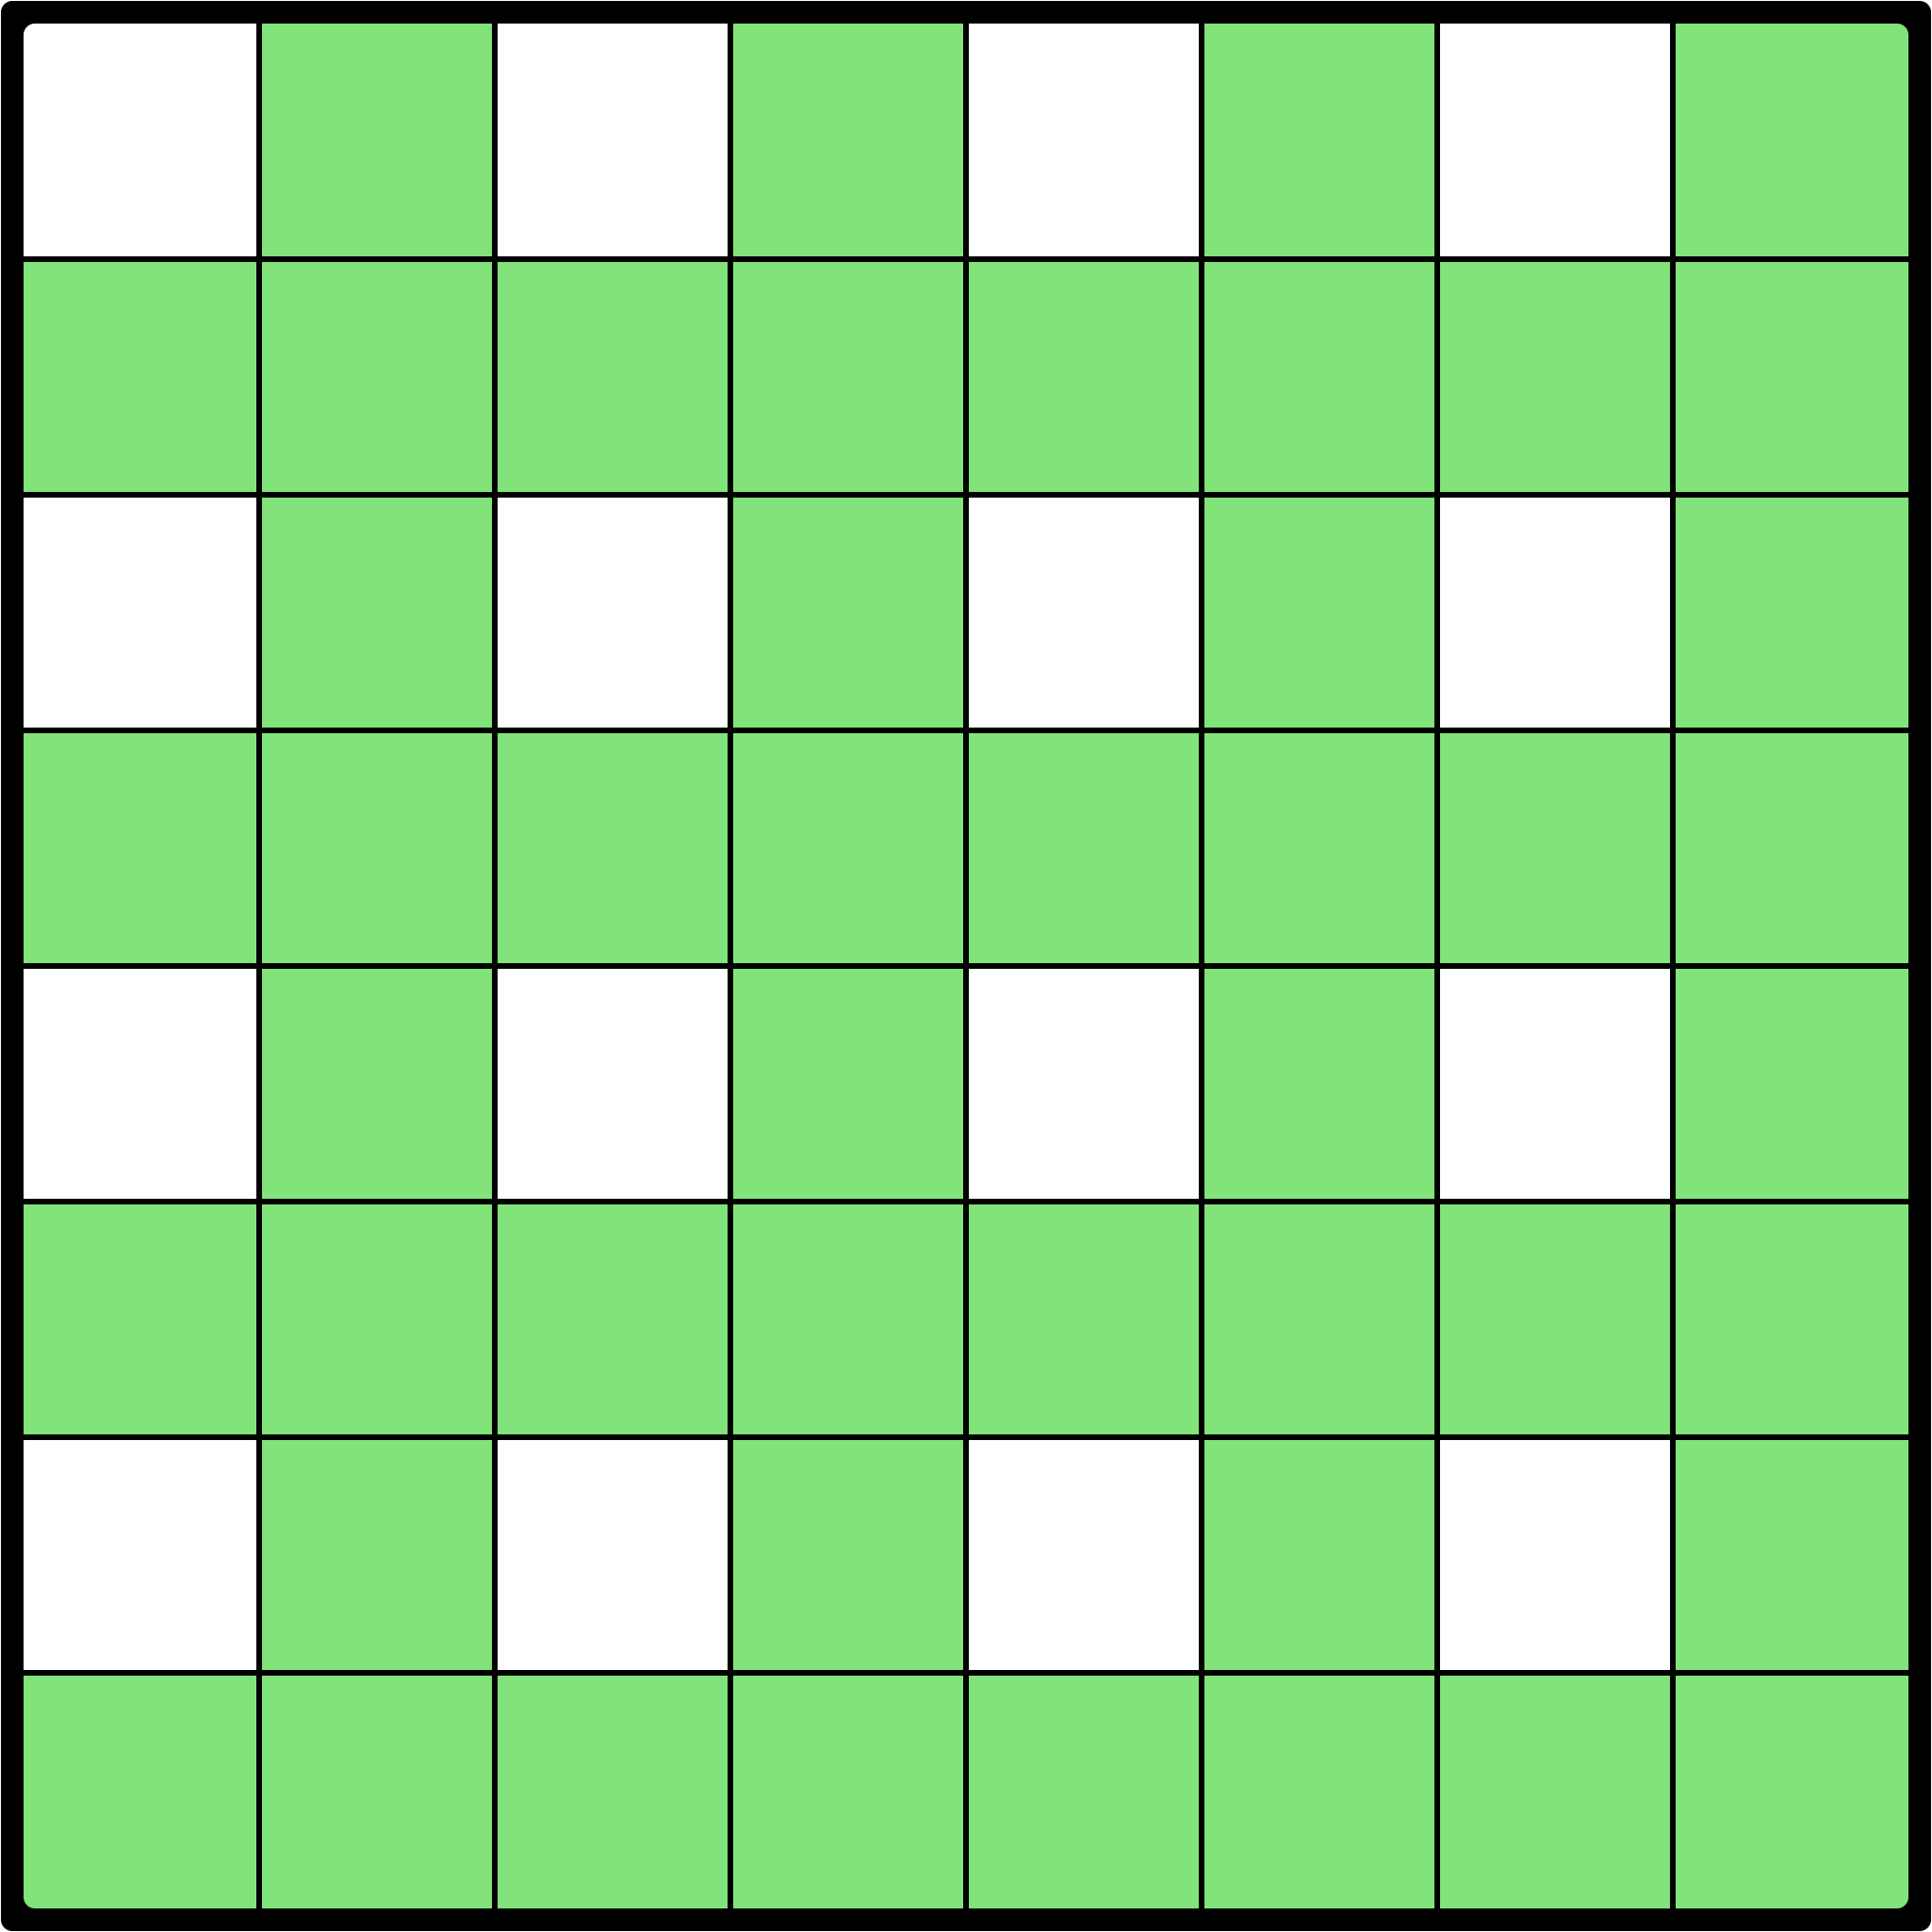
\includegraphics[width=0.45\linewidth]{pics/explaination/explaination-04}
    \captionof{figure}[Erkl\"arung 04]{Nach Terminierung erh\"alt man die erreichbaren Felder Karte (Gr\"un markiert)}
    \label{fig:explaination-04}
\end{minipage}

\subsection{Vorteile durch den MapAnalyzer}\label{subsec:vorteile-mapanalyzer}
Es gibt verschiedene Arten von Vorteilen, die eine genaue Kartenberechnung mit sich bringt.
So erh\"alt man zum Beispiel eine adequate Berechnung, wie viele Felder der Karte bereits belegt sind, da man unerreichbare Bereiche der Karte nicht ber\"ucksichtigt werden.
Des Weiteren kann man durch das Herausrechnen auch verhindern, dass die Kartenbewertung durch Spezialsteine beeinflusst werden, die eigentlich gar nicht erreichbar sind.
Im Folgenden werden nun die beiden Vorteile genauer erl\"autert.

\subsubsection{Leichtere Bewertung des Spielfortschritts}\label{subsubsec:bewertung-fortschritt}
Wenn man sich die Karte aus dem vorherigen Beispiel ansieht, kann man naiv mit der folgenden Formel die Anzahl der unbelegten Felder berechnen.

Bei dem Beispiel aus Abbildung~\ref{fig:explaination-04} ergibt sich folgende Berechnung:
\begin{align}
    (8 \cdot 8) - 3 = 61\; \texttt{Freie Felder}
\end{align}
F\"ur diese Bewertung ist das Spiel zu 5\% abgeschlossen.
In vielen F\"allen werden die 100\% nie erreicht da oft gr\"o"sere Teile nicht erreichbar sind oder das Spiel durch Eliminierung oder Disqualifikation vorzeitig beendet wird.

Im Gegensatz dazu liefert der MapAnalyzer, dass bei diesem Feld maximal 48 Felder bespielbar sind.
Wenn man die beiden bereits belegten abzieht, bleiben noch 45 unbelegte Felder \"ubrig.
Das Spiel ist hier also bereits zu ca. 7\% abgeschlossen.
Nat\"urlich kann es immer noch passieren, dass Felder w\"ahrend eines Spiels nicht erreicht werden, da zum Beispiel zuvor keine Z\"uge mehr m\"oglich sind, doch trotzdem bietet dieses Verfahren die M\"oglichkeit den aktuellen Spielfortschritt besser einzusch\"atzen und somit die Heuristik der K.I.\ exakter anzupassen.

\subsubsection{Herausrechnen von nicht erreichbaren Bonusfeldern}\label{subsubsec:entfernung-bonusfelder}
Wie oben bereits aufgezeigt, sind bei einigen Karten bestimmte Felder nicht erreichbar, dieses Wissen kann f\"ur bestimmte Maps ausgenutzt werden.
Sieht man sich die erreichbaren Felder der Karte in Abbildung~\ref{fig:wall-reachable-01} an, sieht es so aus, als w\"are nur eine Reihe im linken Kartenteil erreichbar.

\vspace{1em}
\begin{minipage}{\linewidth}
    \centering
    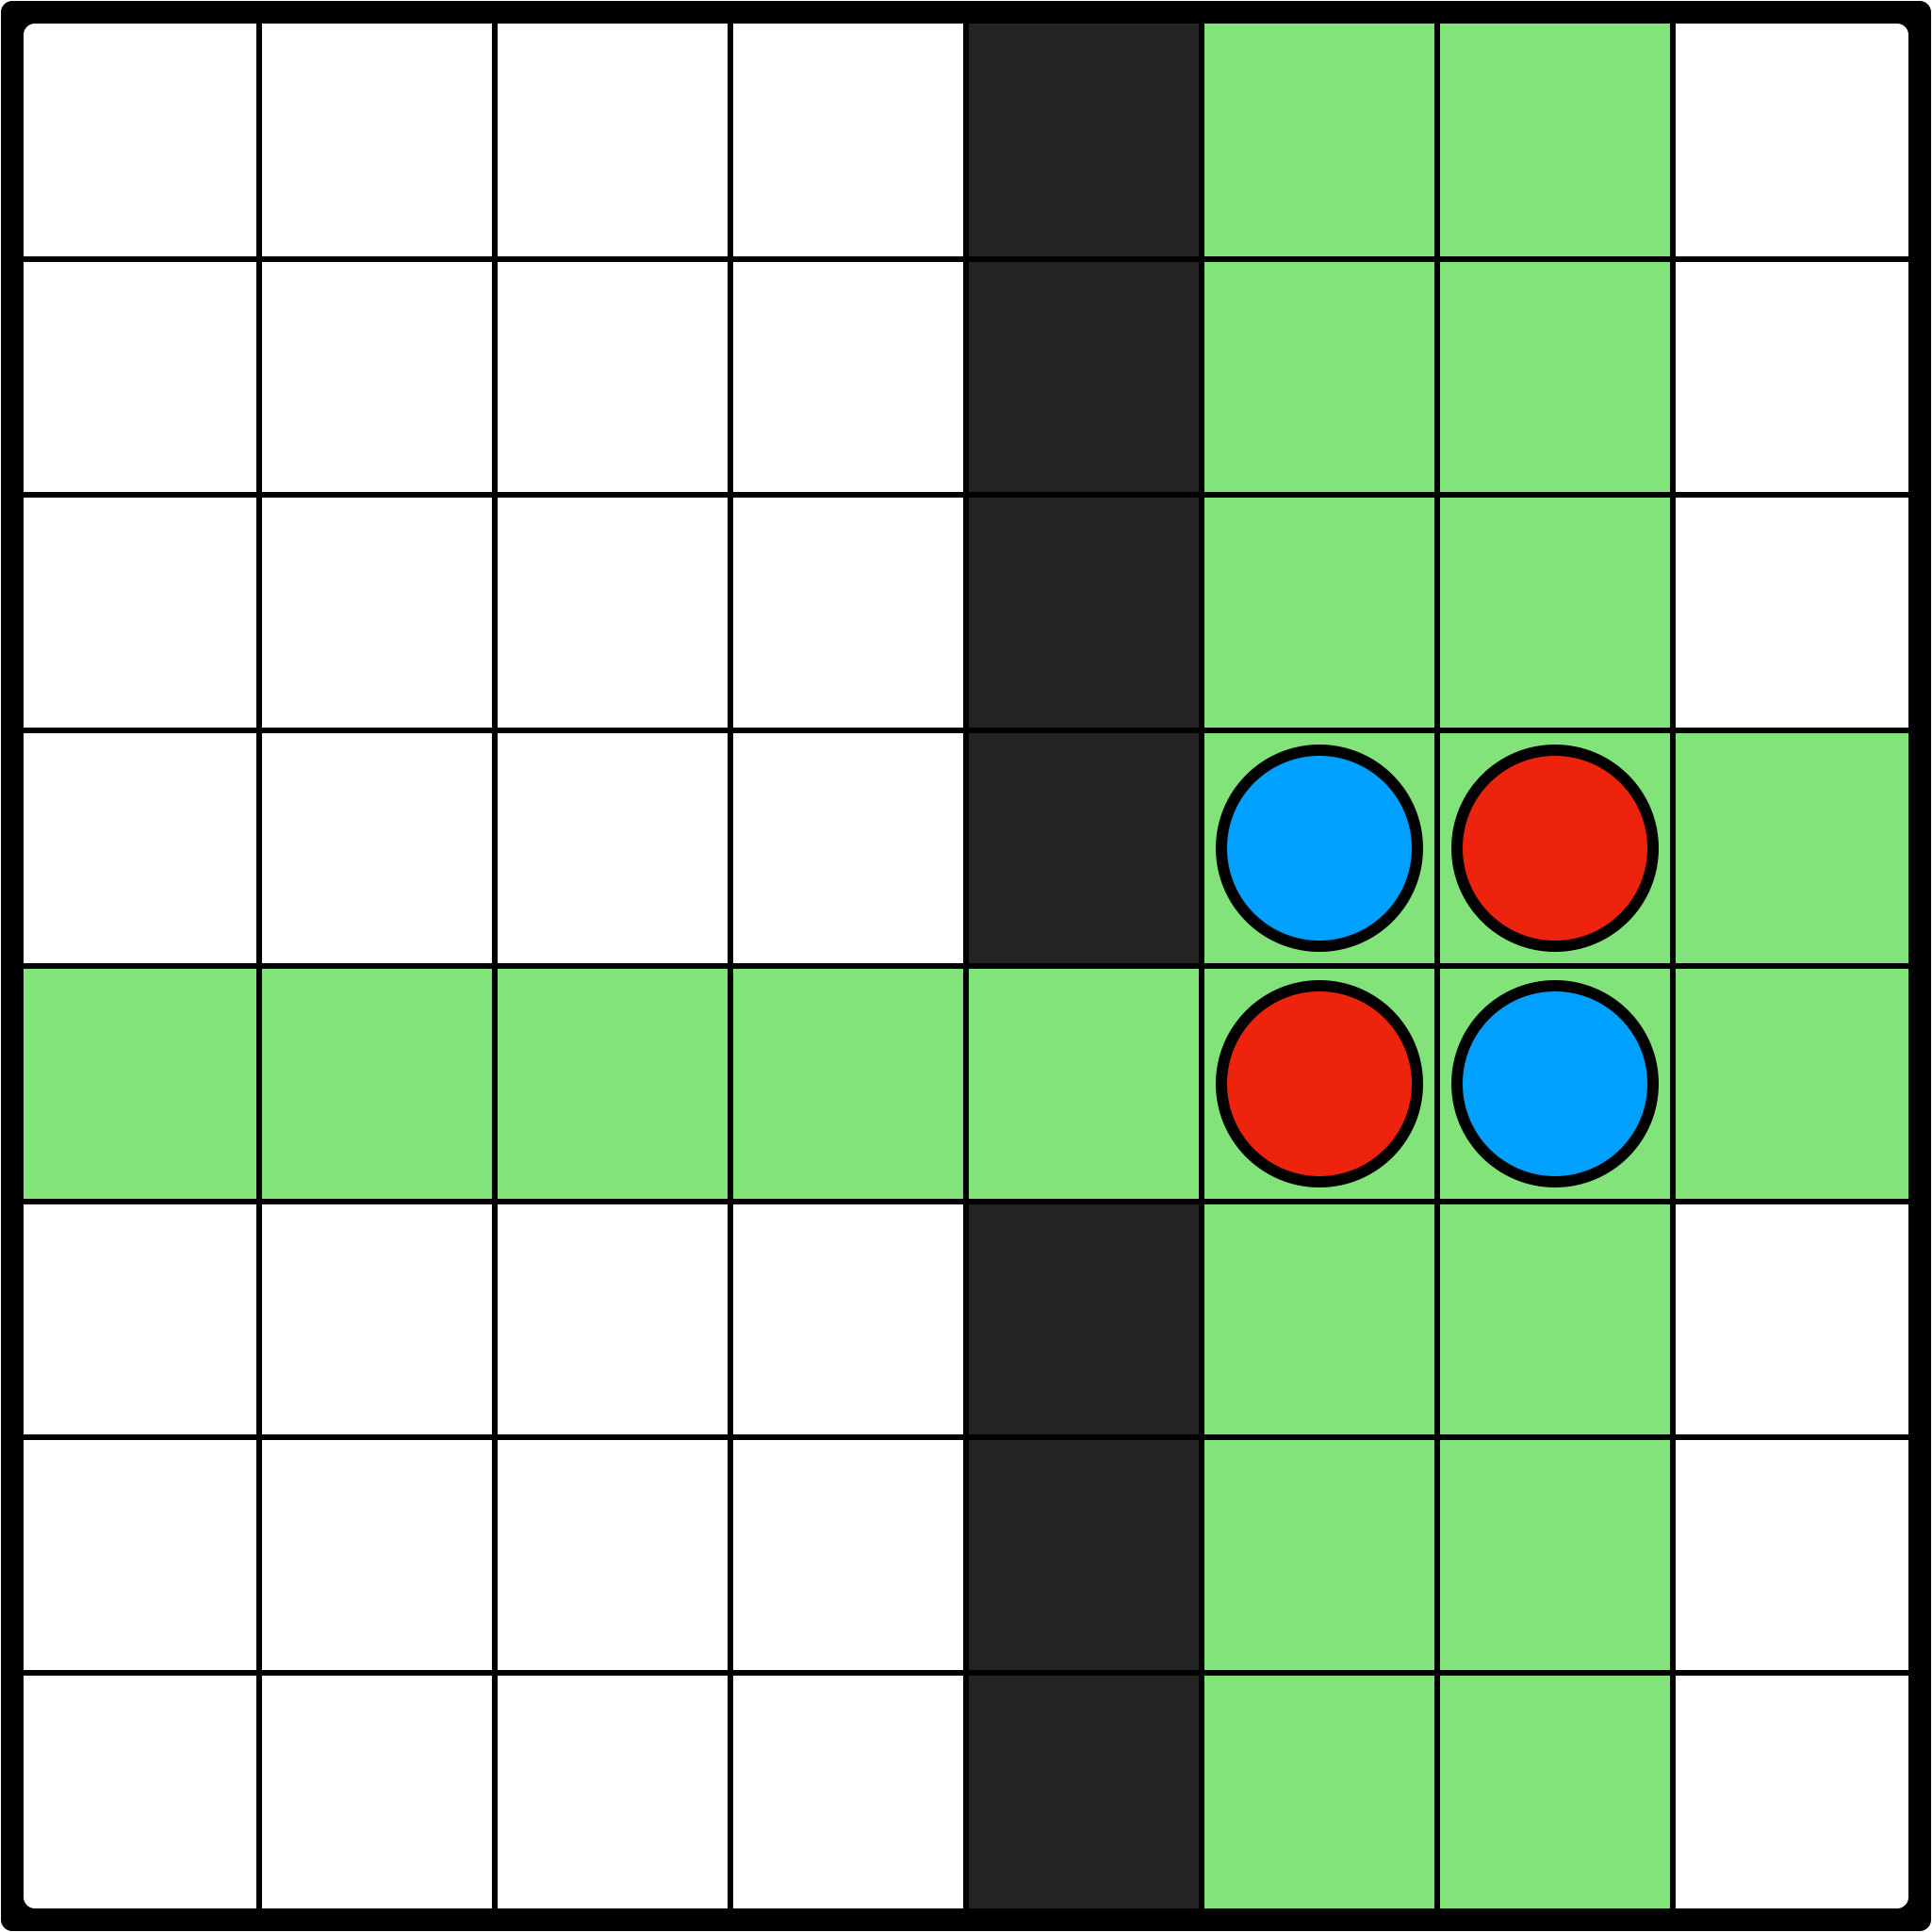
\includegraphics[width=0.45\linewidth]{pics/wall-reachable/wall-reachable-01}
    \captionof{figure}[Sperren durch Wand 01]{Felder die auf den ersten Blick erreichbar sind. (Gr\"un eingezeichnet)}
    \label{fig:wall-reachable-01}
\end{minipage}
\vspace{0.5em}

Wenn man jedoch die n\"achsten M\"oglichkeiten einzeichnet (siehe Abbildung~\ref{fig:wall-reachable-02}), wird schnell ersichtlich, dass mehr Felder erreichbar sind.

\vspace{1em}
\begin{minipage}{\linewidth}
    \centering
    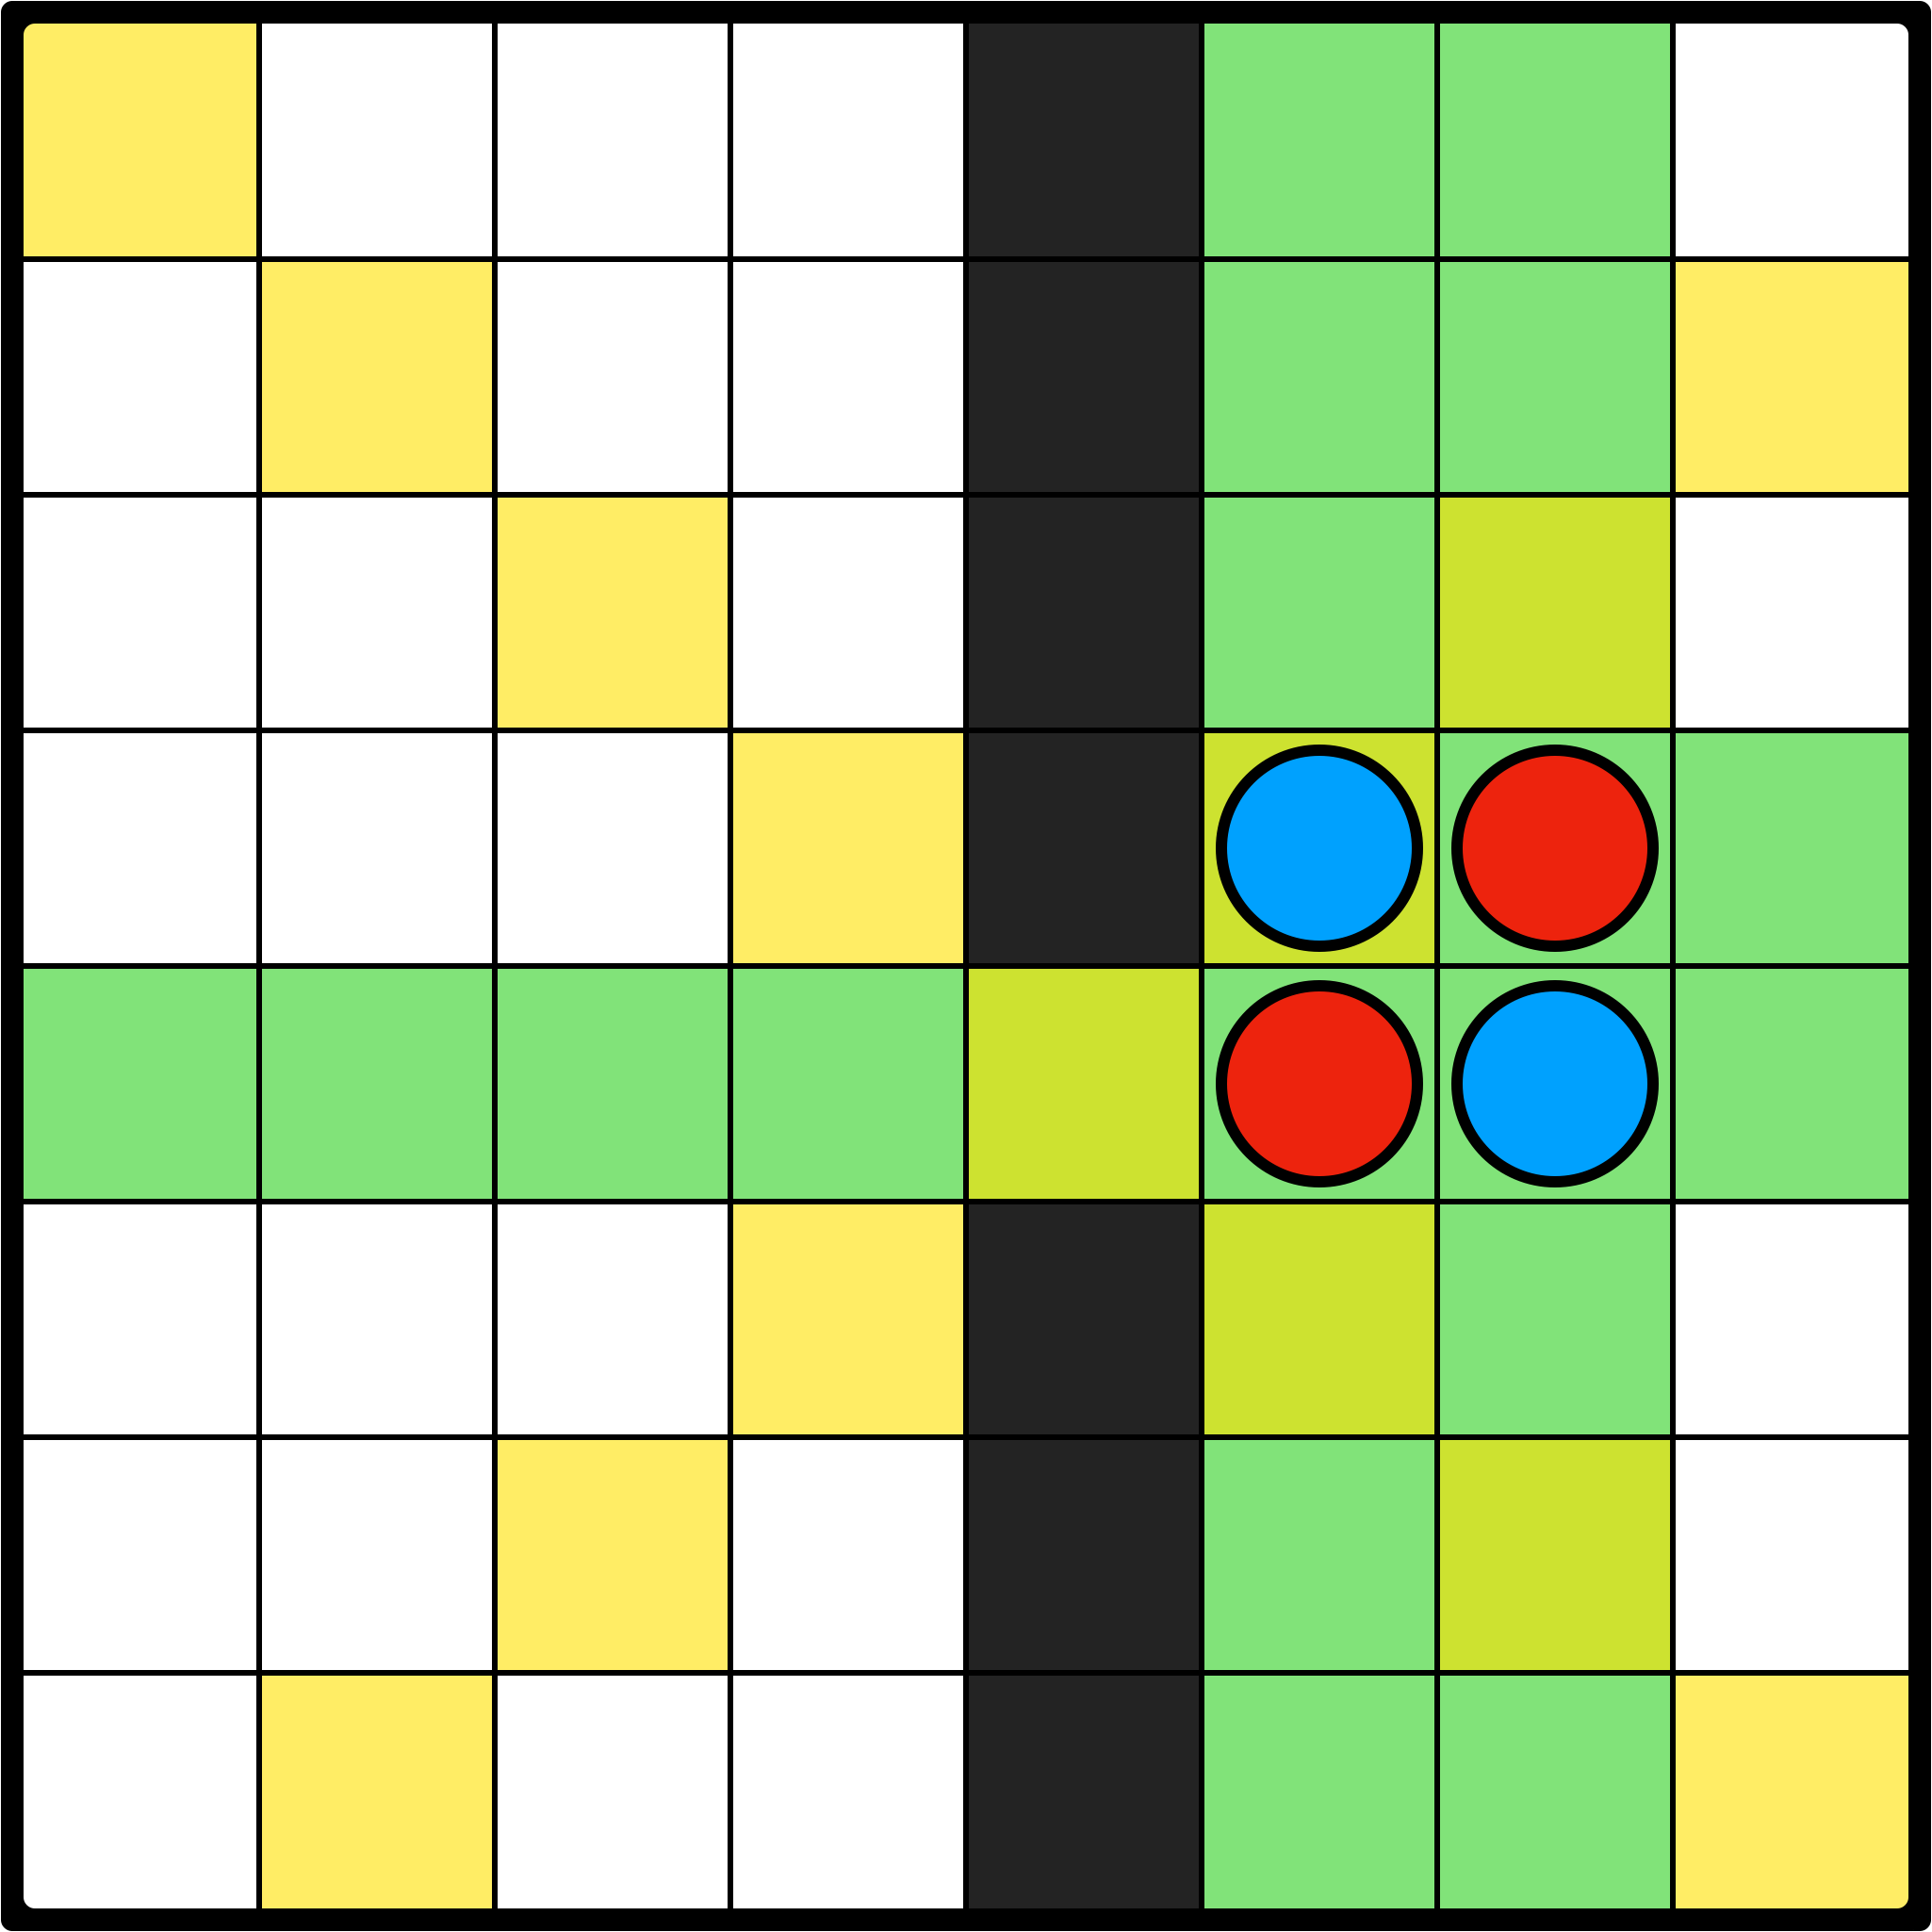
\includegraphics[width=0.45\linewidth]{pics/wall-reachable/wall-reachable-02}
    \captionof{figure}[Sperren durch Wand 02]{Felder die auf den zweiten Blick erreichbar sind. (Gr\"un eingezeichnet)}
    \label{fig:wall-reachable-02}
\end{minipage}
\vspace{0.5em}

Der Algorithmus wird in der Abbildung~\ref{fig:wall-reachable-02} nach dem gleichen Prinzip fortgef\"uhrt.
Dadurch wird ersichtlich, dass in der linken Spielfeldh\"alfte die Felder nur in einem ganz bestimmtem Muster erreichbar sind.

\vspace{1em}
\begin{minipage}{\linewidth}
    \centering
    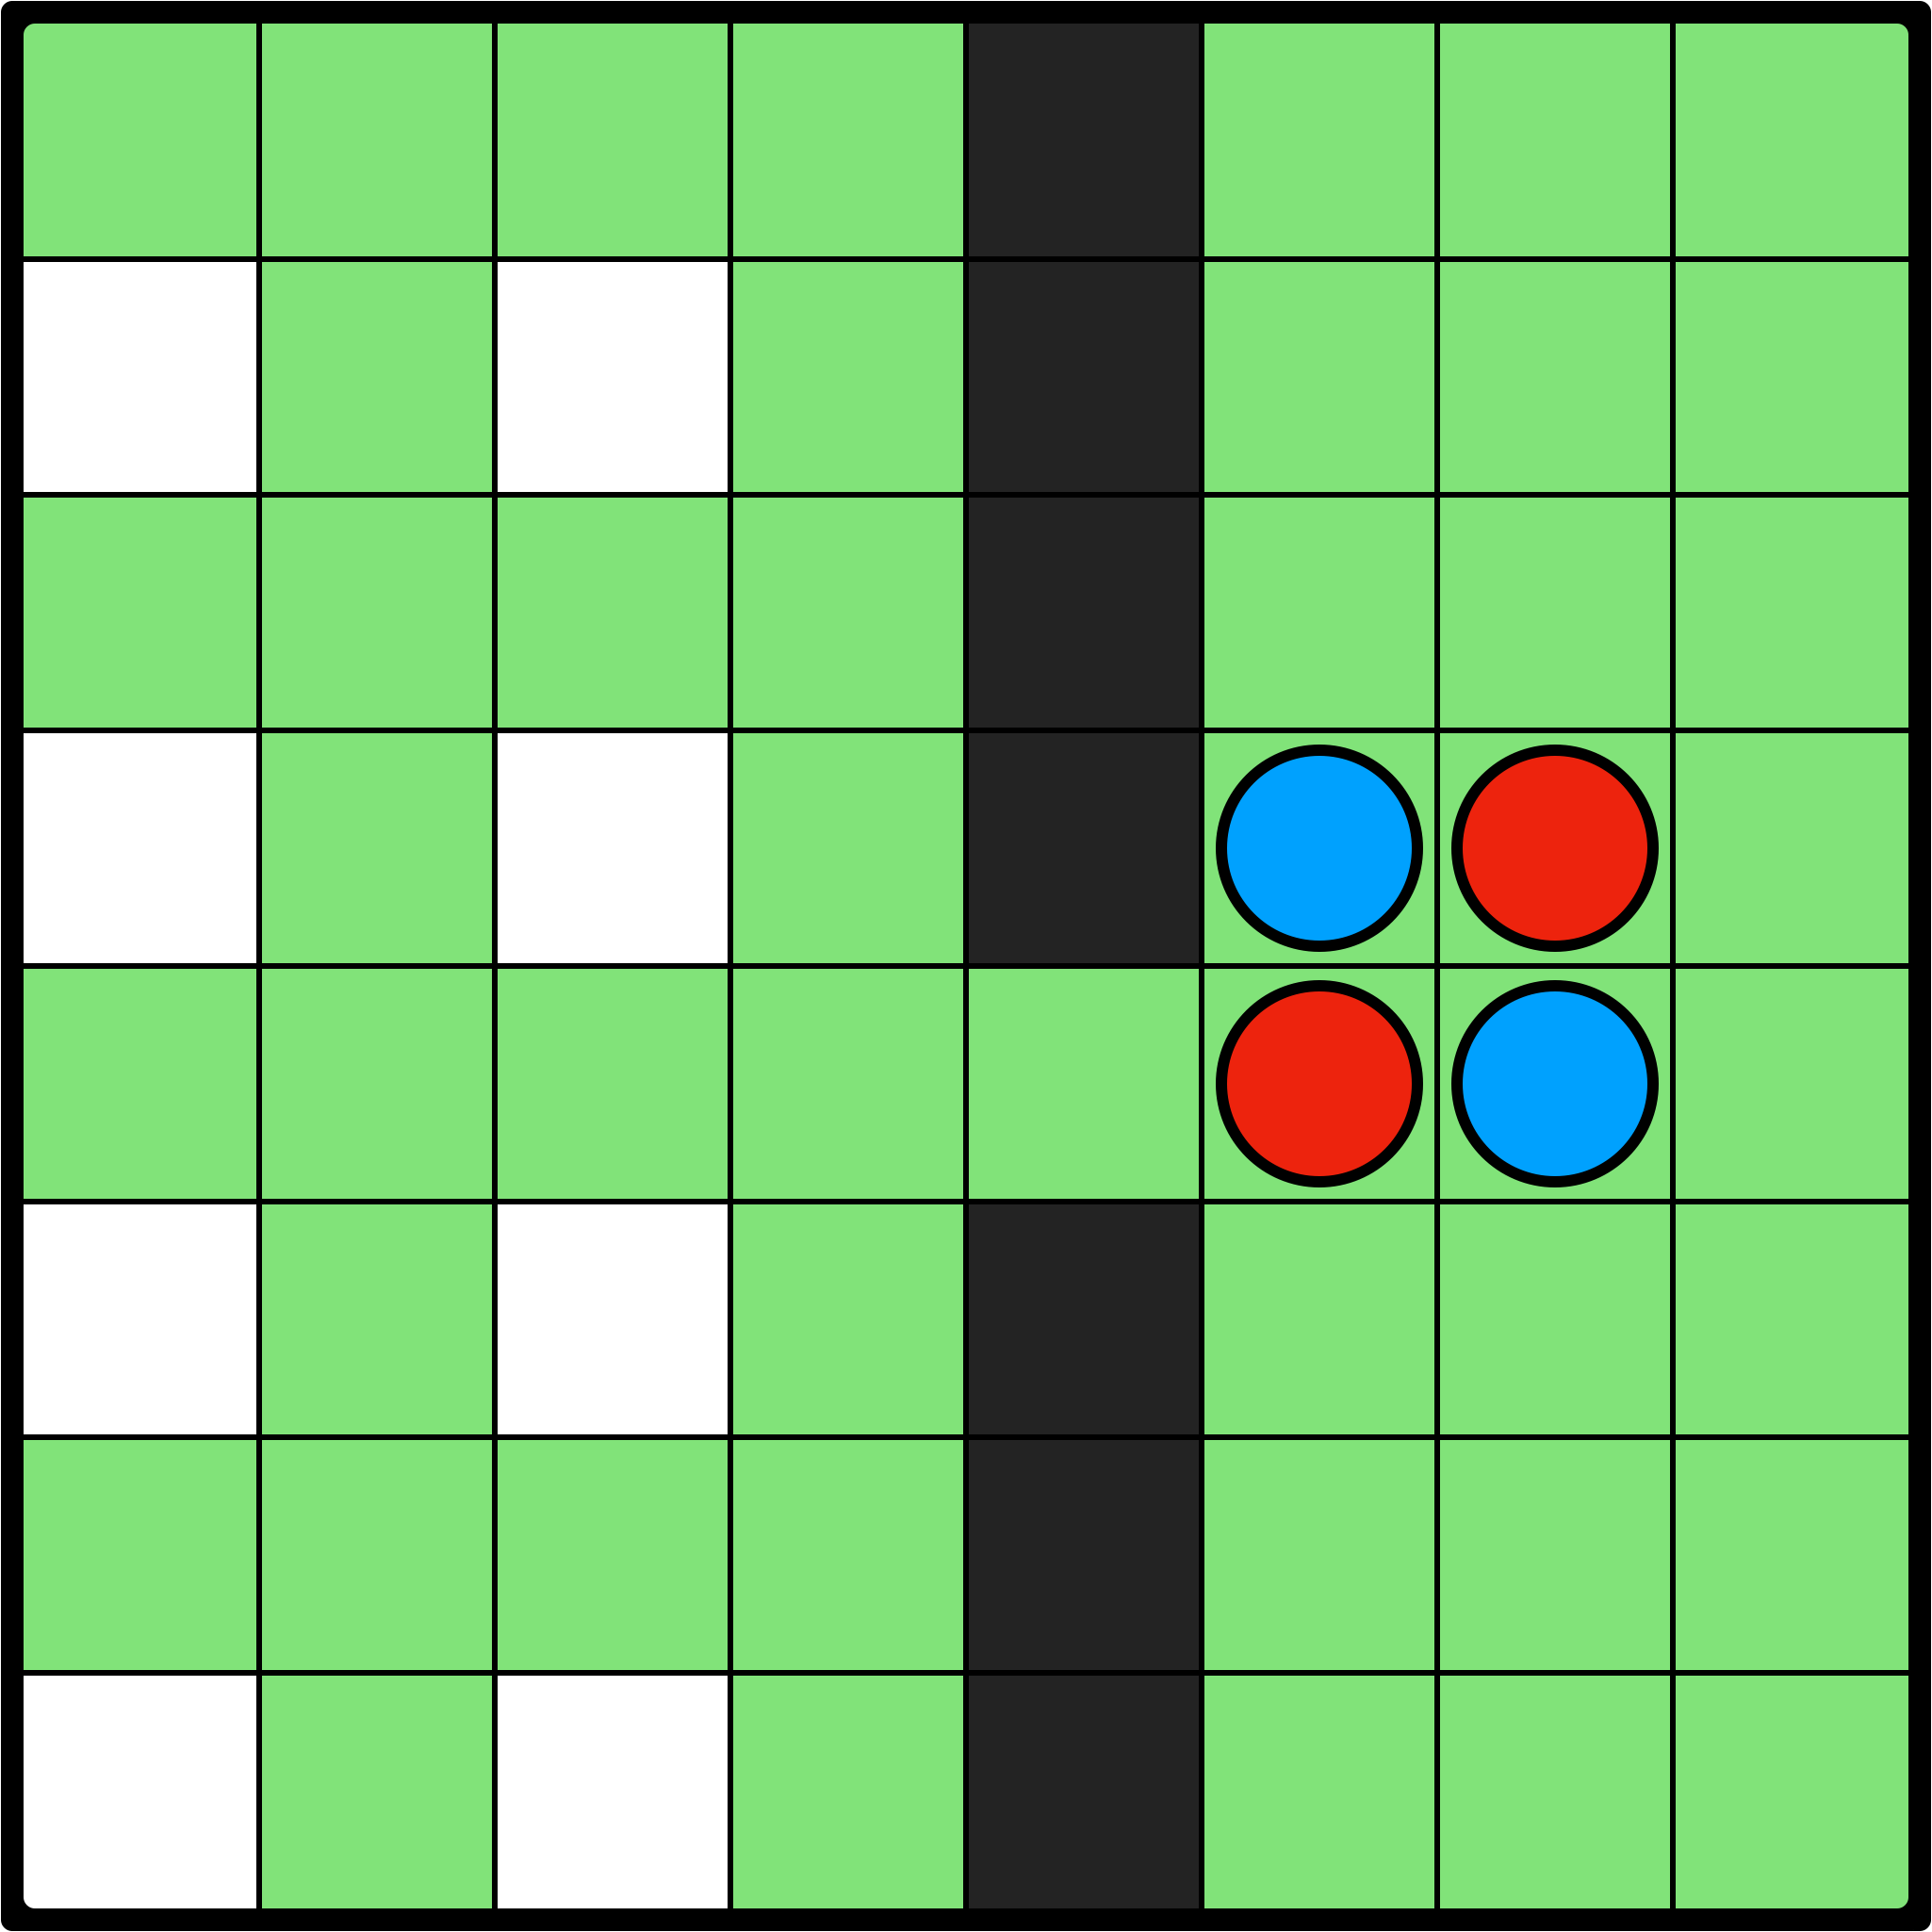
\includegraphics[width=0.45\linewidth]{pics/wall-reachable/wall-reachable-03}
    \captionof{figure}[Sperren durch Wand 03]{Nach Terminierung erh\"alt man die erreichbaren Felder. (Gr\"un markiert)}
    \label{fig:wall-reachable-03}
\end{minipage}
\vspace{0.5em}

Die Strategie ist nun in diese Felder gezielt Spezialsteine zu legen.
Diese Spezialfelder werden durch den MapAnalyzer noch bevor der erste Zug berechnet wird herausgerechnet und bei der Bewertung der Karte unber\"ucksichtigt gelassen.
Dadurch l\"asst sich der Client nicht von \textit{falschen} Bonusfeldern verwirren und hat somit einen Vorteil gegen Clients die auf ein Herausrechnen verzichten.

\subsection{Herausforderung bei der Entwicklung}\label{subsec:herausforderung-mapanalyzer}
Bei der Entwicklung sind zwei gr\"o"sere Probleme deutlich geworden.
Zum einen war ein Problem die Performance, da man nat\"urlich die meiste Zeit in die Berechnung der Z\"uge und nicht in die Analyse der Karte investieren will.
Zum anderen muss die Analyse der Karte auch mit vielen Transitionen fehlerfrei funktionieren.

\subsubsection{Performance Probleme}\label{subsubsec:performance-probleme}
Die ersten Versionen waren rein rekursiv, was bei gr\"o"seren Karten schnell zu einem \"Uberlauf des Speichers gef\"uhrt hat.
Um dieses Problem zu beheben, wurde der Analysevorgang von einem rekursiven Algorithmus zu einem teilweise iterativen Algorithmus umgebaut.
Jedoch ist dies bei gr\"o"seren Karten, die zus\"atzlich sehr viele Transitionen bzw.\ Expansionssteine haben, nach wie vor vorhanden problematisch.
Um dieses Problem zu beheben, muss man verstehen, wie der Map Analyzer bei der Analyse vorgeht.
Wenn s\"amtliche Steine der Karte mit Expansionssteinen belegt sind, f\"uhrt das, weil die Mapanalyse im Uhrzeigersinn abl\"auft, zu einem Zickzack des Algorithmus durch die Karte.
Der iterative Ansatz reduziert die Performance kaum, da die ganze Zeit neue rekursive Aufrufe f\"ur jede neue Richtungen entstehen.
Dieses Problem wurde durch das Vormarkieren von Feldern gel\"ost.
Wenn ein g\"ultiger Zug erkannt wird, werden die Felder in dieser Richtung und der entgegengesetzten Richtung markiert.
Markierte Felder sind hier also Felder die in einer sp\"ateren Iteration noch von der iterativen Funktion durchlaufen werden und deshalb keinen eigenen rekursiven Aufruf ben\"otigen.
Dadurch kann man die Anzahl der rekursiven Aufrufe in einer Karte mit vielen Startsteinen drastisch reduzieren.

\subsubsection{Fehlerfreies abgehen von Transitionen}\label{subsubsec:fehlerfreie-transitionen}
Transitionen erh\"ohen allgemein die Komplexit\"at von ReversiXT enorm und sie stellen w\"ahrend der gesamten Entwicklung eine gro"se Herausforderung da.
Das Problem beim Analysieren der Karte im Zusammenhang mit Transitionen ist das Erkennen von Schleifen die \"uber Transitionen entstehen k\"onnen.
Wie eine \textit{Transitionenschleife} aussehen kann wird in der folgenden Abbildung gezeigt:

\vspace{1em}
\begin{minipage}{\linewidth}
    \centering
    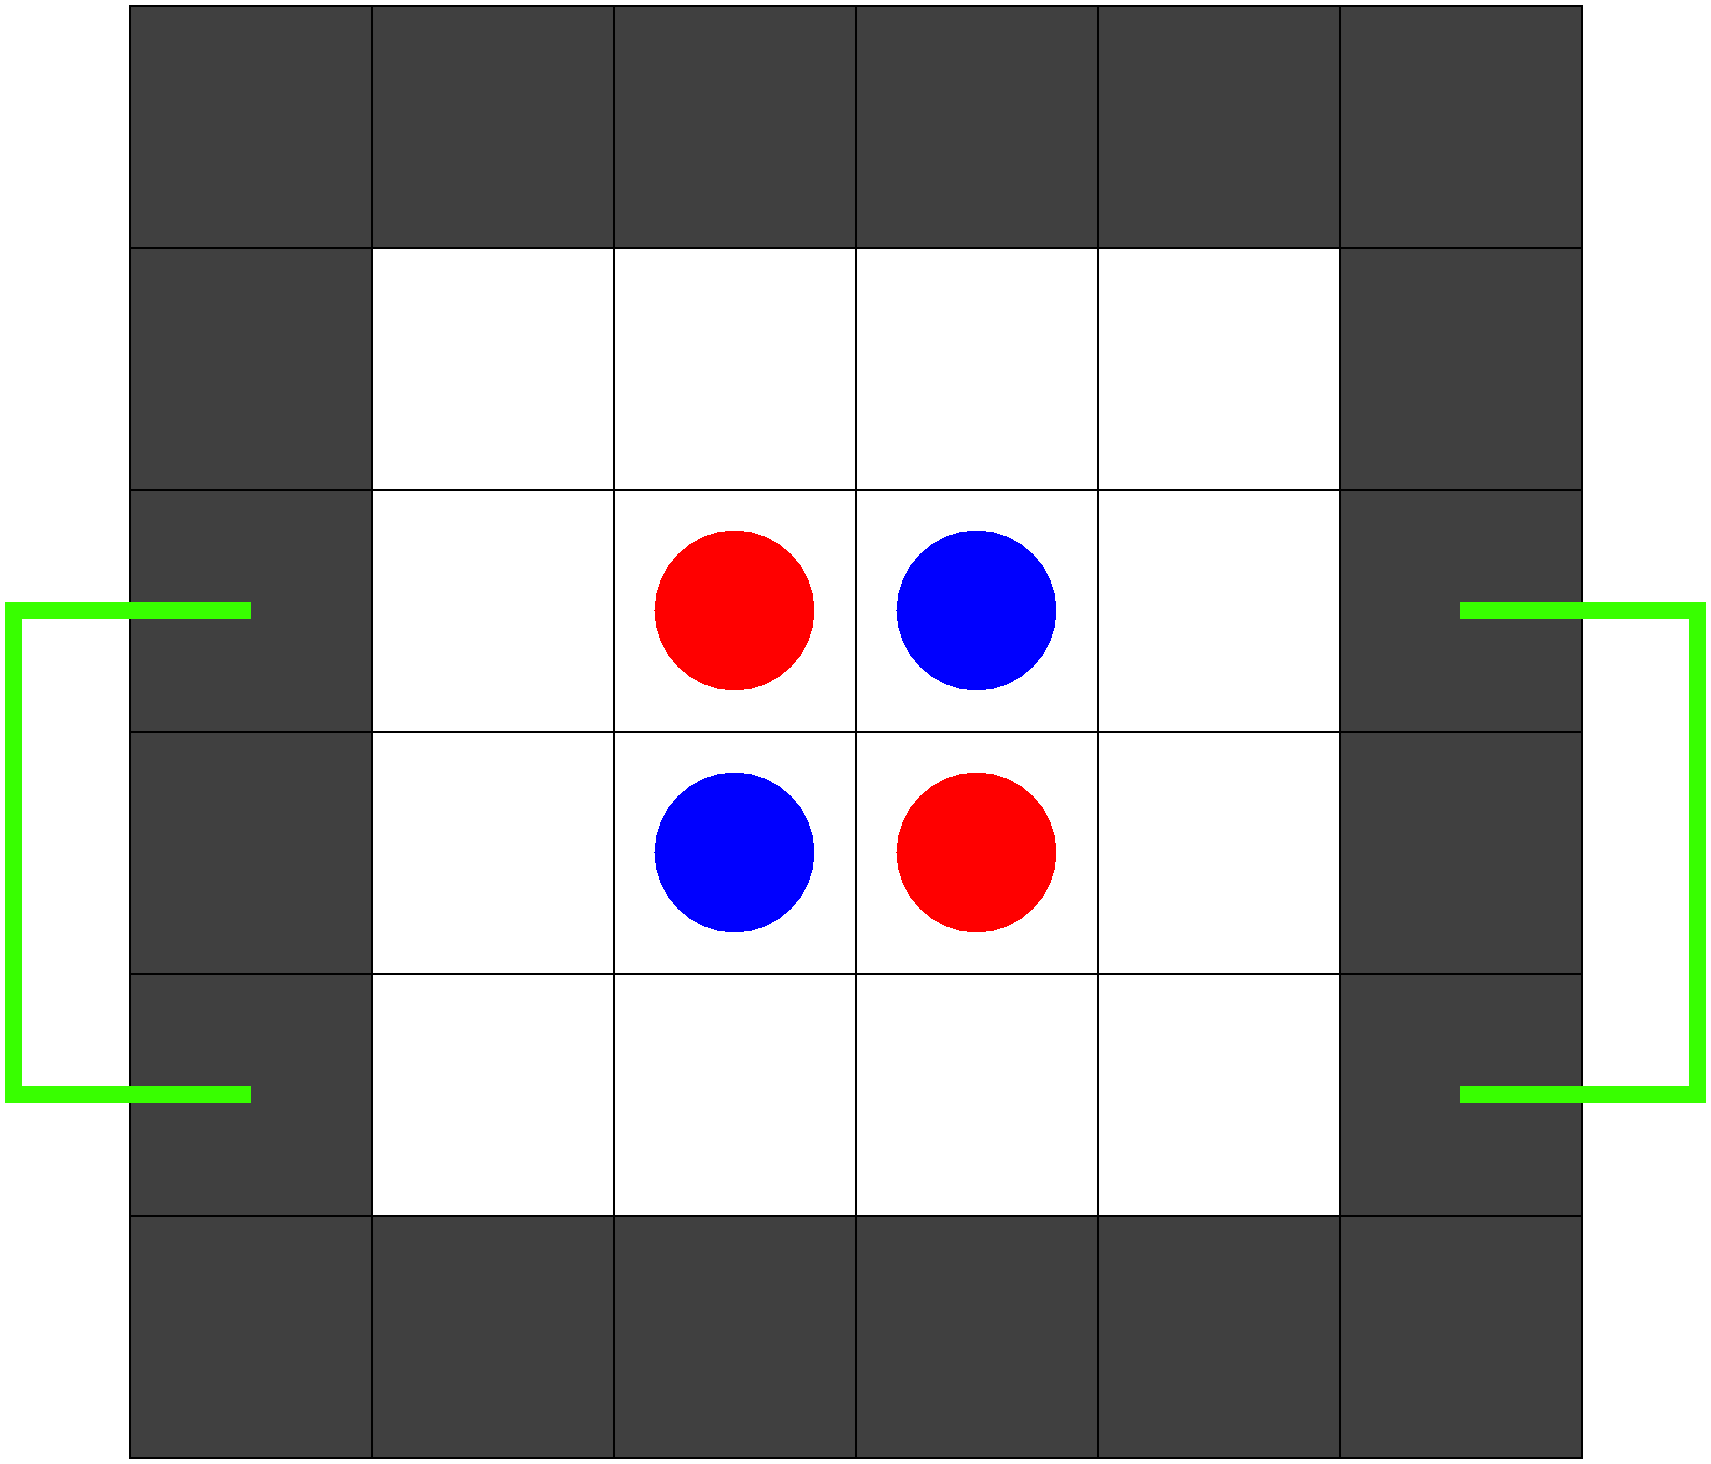
\includegraphics[width=0.3\linewidth]{pics/transition-loop}
    \captionof{figure}[Transitionenschleife]{Darstellung einer Transitionenschleife.}
    \label{fig:transition-loop}
\end{minipage}
\vspace{0.5em}

Es kann also passieren, dass der Algorithmus, welcher die Map analysiert endlos der Transition folgt.
Um das zu verhindern, merkt sich der Algorithmus welche Transitionen bereits abgegangen wurden und benutzt diese kein zweites mal.
Damit k\"onnen Endlosschleifen verhindert werden.
Dadurch erh\"oht sich die Performance, da in sp\"ateren Iterationen alten Transitionen nicht erneut gefolgt werden muss.

\subsubsection{Fehler bei der Berechnung}\label{subsubsec:fehlerhafte-berechnung}
Der MapAnalyzer berechnet alle theoretisch erreichbaren Felder.
Da es aber zum Erreichen neuer Felder immer n\"otig ist, gegnerische Steine oder Expansionssteine zu \"uberziehen, ist in der Realit\"at meistens weniger begehbar als eigentlich m\"oglich ist.
Der MapAnalyzer ist bei der Analyse optimistisch, das hei"st es wird lieber angenommen, dass ein Feld welches nicht erreichbar ist, als erreichbar angezeigt wird, als das Felder die erreichbar sind als nicht erreichbar eingestuft werden.
Dies w\"urde f\"ur die Zugberechnung fatale Folgen haben, da dadurch m\"ogliche Z\"uge nicht erkannt werden.

\bigskip
\newpage